%%%%%%%% ICML 2026 EXAMPLE LATEX SUBMISSION FILE %%%%%%%%%%%%%%%%%

\documentclass{article}

% Recommended, but optional, packages for figures and better typesetting:
\usepackage{microtype}
\usepackage{graphicx}
\usepackage{subcaption}
\usepackage{float} % for precise figure placement
\usepackage{booktabs} % for professional tables
\usepackage{multirow}
\usepackage{colortbl}

% hyperref makes hyperlinks in the resulting PDF.
% If your build breaks (sometimes temporarily if a hyperlink spans a page)
% please comment out the following usepackage line and replace
% \usepackage{icml2026} with \usepackage[nohyperref]{icml2026} above.
\usepackage{hyperref}


% Attempt to make hyperref and algorithmic work together better:
\newcommand{\theHalgorithm}{\arabic{algorithm}}

% Use the following line for the initial blind version submitted for review:
% \usepackage{icml2026}

% For preprint, use
\usepackage{icml2026}

% If accepted, instead use the following line for the camera-ready submission:
% \usepackage{icml2026}

\usepackage{amsmath}
\usepackage{amssymb}
\usepackage{mathtools}
\usepackage{amsthm}
\usepackage{bbm}
\usepackage{pifont}
\newcommand{\cmark}{\ding{51}}
\newcommand{\xmark}{\ding{55}}


% if you use cleveref..
\usepackage[capitalize,noabbrev]{cleveref}

%%%%%%%%%%%%%%%%%%%%%%%%%%%%%%%%
% CUSTOM BOXES
%%%%%%%%%%%%%%%%%%%%%%%%%%%%%%%%
\usepackage{tcolorbox}
\tcbuselibrary{skins}

\definecolor{facOrange}{HTML}{FAC074}
\definecolor{skyBlue}{HTML}{6C8EBF}

\newtcolorbox{defaultbox}{
  enhanced,
  arc=4mm,
  colback=gray!10,
  colframe=black,
  boxrule=1pt,
  left=6pt, right=6pt,
  top=6pt, bottom=6pt,
}

\newtcolorbox{orangebox}{
  enhanced,
  arc=4mm,
  colback=gray!10,
  colframe=facOrange,
  boxrule=1pt,
  left=6pt, right=6pt,
  top=6pt, bottom=6pt,
}

\newtcolorbox{bluebox}{
  enhanced,
  arc=4mm,
  colback=gray!10,
  colframe=skyBlue,
  boxrule=1pt,
  left=6pt, right=6pt,
  top=6pt, bottom=6pt,
}

\newcommand{\SL}[1]{{\textcolor{red}{SL: #1}}}

%%%%%%%%%%%%%%%%%%%%%%%%%%%%%%%%
% THEOREMS
%%%%%%%%%%%%%%%%%%%%%%%%%%%%%%%%
\theoremstyle{plain}
\newtheorem{theorem}{Theorem}[section]
\newtheorem{proposition}[theorem]{Proposition}
\newtheorem{lemma}[theorem]{Lemma}
\newtheorem{corollary}[theorem]{Corollary}
\theoremstyle{definition}
\newtheorem{definition}[theorem]{Definition}
\newtheorem{assumption}[theorem]{Assumption}
\theoremstyle{remark}
\newtheorem{remark}[theorem]{Remark}
\newtheorem{example}[theorem]{Example}

% Todonotes is useful during development; simply uncomment the next line
%    and comment out the line below the next line to turn off comments
%\usepackage[disable,textsize=tiny]{todonotes}
\usepackage[textsize=tiny]{todonotes}

% The \icmltitle you define below is probably too long as a header.
% Therefore, a short form for the running title is supplied here:
\icmltitlerunning{RC-GRPO: Reward-Conditioned Group Relative Policy Optimization for Multi-Turn Tool Calling Agents}

\begin{document}

\twocolumn[
  \icmltitle{RC-GRPO: Reward-Conditioned Group Relative Policy Optimization for Multi-Turn Tool Calling Agents}

  % It is OKAY to include author information, even for blind submissions: the
  % style file will automatically remove it for you unless you've provided
  % the [accepted] option to the icml2026 package.

  % List of affiliations: The first argument should be a (short) identifier you
  % will use later to specify author affiliations Academic affiliations
  % should list Department, University, City, Region, Country Industry
  % affiliations should list Company, City, Region, Country

  % You can specify symbols, otherwise they are numbered in order. Ideally, you
  % should not use this facility. Affiliations will be numbered in order of
  % appearance and this is the preferred way.
  \icmlsetsymbol{equal}{*}

  \begin{icmlauthorlist}\icmlauthor{Anonymous}{anon}\end{icmlauthorlist}

  \icmlaffiliation{anon}{Anonymous Institution}
  
  
  
  
  


%   \icmlcorrespondingauthor{Anonymous}{anonymous@anonymous.invalid}
  
%   

  % You may provide any keywords that you find helpful for describing your
  % paper; these are used to populate the "keywords" metadata in the PDF but
  % will not be shown in the document
  \icmlkeywords{Large Language Models, Reinforcement Learning, Tool Calling, Multi-turn Agents, Policy Optimization, Decision Transformer}

  \vskip 0.3in
]

% this must go after the closing bracket ] following \twocolumn[ ...

% This command actually creates the footnote in the first column listing the
% affiliations and the copyright notice. The command takes one argument, which
% is text to display at the start of the footnote. The \icmlEqualContribution
% command is standard text for equal contribution. Remove it (just {}) if you
% do not need this facility.

% Use ONE of the following lines. DO NOT remove the command.
% If you have no special notice, KEEP empty braces:
\printAffiliationsAndNotice{}  % no special notice (required even if empty)
% Or, if applicable, use the standard equal contribution text:
% \printAffiliationsAndNotice{\icmlEqualContribution}
\begin{abstract}
Multi-turn tool calling is challenging for Large Language Models (LLMs) because rewards are sparse and exploration is expensive. A common recipe, SFT followed by GRPO, can stall when within-group reward variation is low (e.g., more rollouts in a group receive the all 0 or all 1 reward), making the group-normalized advantage uninformative and yielding vanishing updates. To address this problem, we propose \textbf{RC-GRPO} (Reward-Conditioned Group Relative Policy Optimization), which treats exploration as a controllable steering problem via discrete reward tokens. We first fine-tune a Reward-Conditioned Trajectory Policy (RCTP) on mixed-quality trajectories with reward goal special token (e.g., \texttt{<|high\_reward|>}, \texttt{<|low\_reward|>}) injected into the prompts, enabling the model to learn how to generate distinct quality trajectories on demand. Then during RL, we sample diverse reward tokens within each GRPO group and condition rollouts on the sampled token to improve within-group diversity, improving agvantage gains. On the Berkley Function Calling Leaderboard v4 (BFCLv4) multi-turn benchmark, our method yields consistantly improved performance than baselines, and the performance on Qwen-2.5-7B-Instruct even surpasses all closed-source API models.
\end{abstract}

\begin{figure*}[!t]
  \centering
  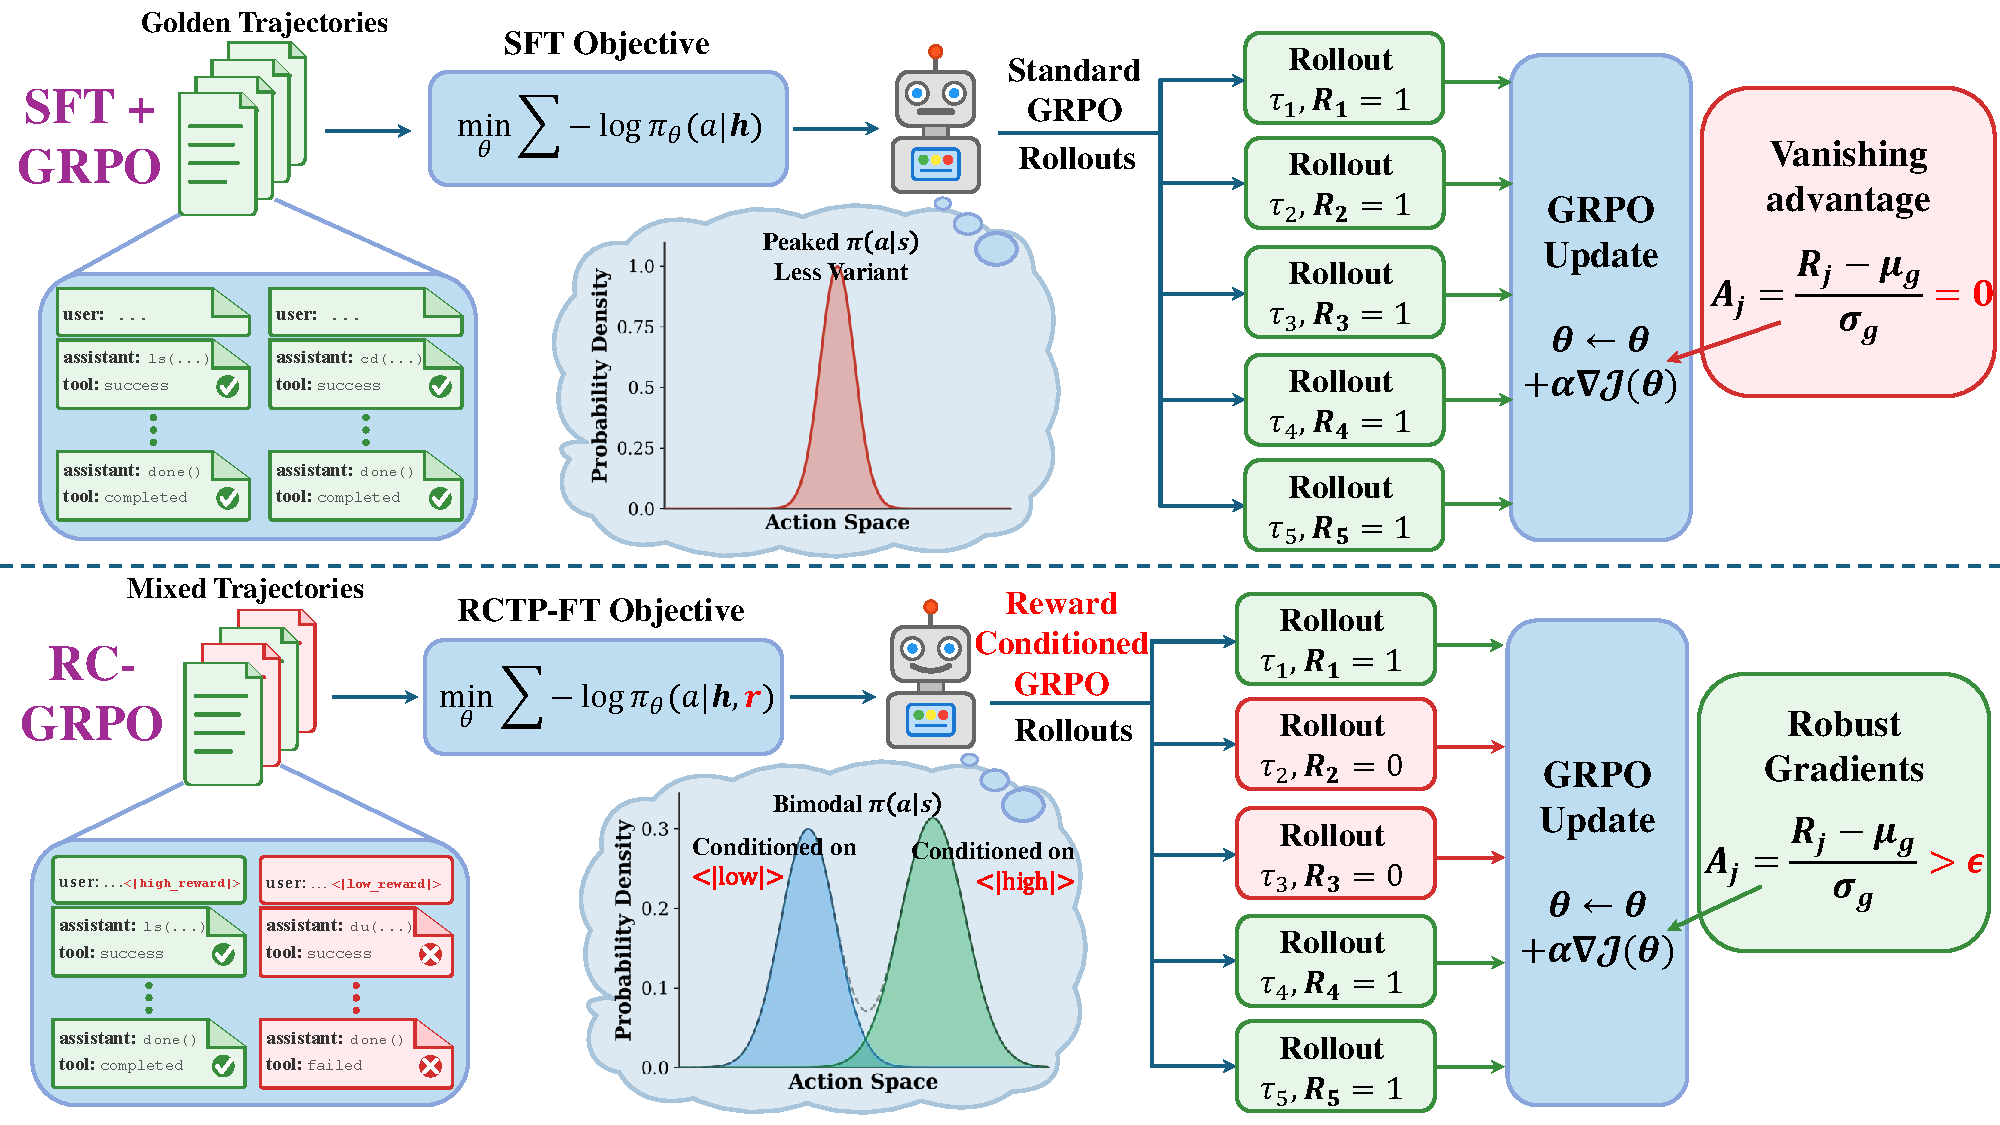
\includegraphics[width=\textwidth]{figure.pdf}
  \caption{Overview of RC-GRPO. \textbf{(Top)} Standard GRPO optimization from an SFT initialization can sharply reduce rollout diversity, yielding low within-group reward variance and a weak/vanishing advantage signal. \textbf{(Bottom)} Our RC-GRPO conditions rollouts on discrete reward tokens and samples diverse tokens within each group, explicitly injecting variance and producing informative advantages.}
  \label{fig:overview}
\end{figure*}

\section{Introduction}
\label{sec:intro}

Tool-using Large Language Models (LLMs) can execute complex tasks by interleaving natural language reasoning with external API calls \cite{yao2023react,schick2023toolformer,gorilla2023,qin2023toolllm}. However, for multi-turn tool calling, success is often measured by sparse, trajectory-level rewards, making exploration costly. In this setting, group-relative policy-gradient methods such as Group Relative Policy Optimization (GRPO) are attractive because they avoid a critic, but their learning signal fundamentally depends on within-group variability: if the rewards within a sampled group have near-zero or even completely zero standard deviation, the group-normalized advantage becomes degenerate and policy updates vanish.

A practical failure mode then appears in the standard SFT-then-GRPO pipeline. SFT on optimal demonstrations intentionally produces a peaked policy (a strong ``golden-path'' prior), which reduces rollout diversity and can substantially reduce within-group reward variance under GRPO. This ``paradox of perfection'' is especially severe for multi-turn tool calling with partial observability \cite{kaelbling1998planning,sutton2018reinforcement}: a policy that is locally confident can repeatedly generate the same short-horizon behavior, leaving little informative contrast for group-relative advantages, consistent with recent analyses of vanishing updates when reward variability under the current policy is small \cite{razin2024vanishing}.

We propose \textbf{RC-GRPO} (Reward-Conditioned Group Relative Policy Optimization), which makes within-group diversity a controlled variable rather than a byproduct of sampling temperature. Inspired by return-conditioned generation \cite{chen2021decision,schmidhuber2019reinforcement}, we first train a Reward-Conditioned Trajectory Policy (RCTP) on mixed-quality trajectories so that the policy can reliably produce distinct behaviors under different tokens; then, during RL with GRPO, we sample diverse reward tokens within each group and condition rollouts on the sampled token, explicitly injecting variance and systematically restoring non-degenerate group-relative advantages.

Our principal contributions are summarized as follows.

\begin{itemize}
    \item We propose \textbf{RC-GRPO}. We first fine-tune a Reward-Conditioned Trajectory Policy (RCTP) on mixed-quality trajectories by appending a reward-goal special token to the prompt, so the policy learns to generate systematically different-quality trajectories under different tokens. We then train the model with reward-conditioned GRPO (RC-GRPO), where each GRPO group samples diverse reward tokens and conditions rollouts on them, ensuring non-degenerate within-group reward variation for group-normalized updates.
    \item We conduct a series of experiments on Berkley Function Calling Leaderboard v4 multi-turn tool calling split using LLaMA-3.1-8B-Instruct and Qwen2.5-7B-Instruct, and we report comparisons against standard SFT+GRPO baselines as well as several strong closed API models .
    \item We analyze training dynamics to justify whether improvements are attributable to increased randomness (entropy trajectories and entropy--reward correlation) and to quantify within-group learning signal quality (advantage spread with KL/gradient statistics). We further provide a variance-based theoretical analysis.
\end{itemize}


\section{Related Work}

\subsection{Tool-Calling LLMs and Benchmarks}
The capability of LLMs to use tools has been evaluated by benchmarks including the Berkeley Function Calling Leaderboard (BFCLv4) \cite{bfcl2024,gorilla2023}, API-Bank \cite{li2023apibank}, and ToolRL \cite{toolrl2024}. We focus on BFCLv4's multi-turn subset, which requires agents to maintain state across sequential tool calls to solve complex queries. In contrast, many tool-use benchmarks (e.g., ToolBench \cite{xu2023toolbench}) primarily evaluate single-turn function selection or parameter correctness without requiring persistent state tracking.

Toolformer \cite{schick2023toolformer} pioneered self-supervised tool learning, while ReAct \cite{yao2023react} introduced interleaved reasoning and acting. ToolLLM \cite{qin2023toolllm} scaled tool-use training to large collections of real-world APIs. While prompt engineering and standard SFT have shown promise, they often struggle with error recovery and long-horizon reasoning. Recent work focuses on closed-loop agents \cite{xi2023rise,wang2024executable}, which is closely related to our setting.

\subsection{RL-based Policy Optimization for LLMs}
Proximal Policy Optimization (PPO) \cite{schulman2017proximal} has been the standard RL algorithm for RLHF \cite{ouyang2022training,stiennon2020learning}. However, PPO requires a separate value network (critic), which doubles the memory footprint. GRPO \cite{deepseek2025r1} removes the critic by estimating advantages relative to a group of outputs generated from the same prompt, reducing memory by $\sim$50\%. Direct Preference Optimization (DPO) \cite{rafailov2023direct} similarly avoids explicit reward modeling but requires pairwise preferences.

Recent work has highlighted unique challenges in \emph{multi-turn} agent RL. RAGEN \cite{wang2025ragen} identifies the ``Echo Trap'' phenomenon where agents overfit to locally rewarded reasoning patterns, proposing trajectory-level rewards. SimpleTIR \cite{wang2025simpletir} addresses training instability from tool feedback deviating from pretrained distributions by filtering void turns during GRPO. Agentic RL with Implicit Step Rewards \cite{putta2025agentic} tackles sparse reward credit assignment via implicit process reward models. Agent Early Experience \cite{zhang2024agent} demonstrates that LLMs can perform model-based planning when fine-tuned to predict environment states.

\subsection{Return-Conditioned Learning}
Return-Conditioned Learning approaches, such as Decision Transformers \cite{chen2021decision} and Upside-Down RL \cite{schmidhuber2019reinforcement}, reframe reinforcement learning as a sequence modeling problem. Instead of estimating value functions or policy gradients, these methods learn a conditional policy $\pi(a|s, R)$ where $R$ represents the target return. During inference, the model is conditioned on a high return value to generate optimal trajectories. This paradigm has been extended to offline RL settings by the Trajectory Transformer \cite{janner2021offline}, which models the joint distribution of states, actions, and rewards. 


\section{Method}
\label{sec:method}

Our method is motivated by a practical pathology observed when applying group-based policy optimization to strong tool-using LLMs. Starting from a high-quality SFT policy, rollouts within a GRPO group can become nearly identical, reducing intra-group reward variance and weakening the relative-advantage signal. In Sec.~\ref{sec:theory} (Q4 in Sec.~\ref{sec:experiments}), we formalize this ``gradient collapse'' phenomenon and show how reward-conditioned rollout generation restores within-group variance without requiring high policy entropy.

In Sec.~\ref{sec:preliminaries}, we first formalize multi-turn tool calling as a POMDP and introduce our reward-conditioned policy parameterization.
Sec.~\ref{sec:stage1} then describes Stage~1, where we fine-tune a Reward-Conditioned Trajectory Policy (RCTP) on mixed trajectories labeled by discrete reward tokens.
Sec.~\ref{sec:rcgrpo} presents Stage~2, where we optimize the policy using GRPO with reward-conditioned sampling to maintain within-group diversity.

\subsection{Preliminaries}
\label{sec:preliminaries}
We formalize multi-turn tool calling as a Partially Observable Markov Decision Process (POMDP). The agent interacts with the environment until episode termination. At each turn $t \in \{1, \ldots, T_{\text{max}}\}$, the user provides a natural language query $u_t$, and the agent generates an action $a_t$, a JSON-formatted tool call containing \texttt{name} and \texttt{args} fields. The environment executes this call and returns an observation $o_t$. The episode terminates when the agent invokes a termination action (e.g., \texttt{done()}) or reaches the maximum turn limit. The history $h_t = (u_0, a_0, o_0, \dots, u_{t-1}, a_{t-1}, o_{t-1}, u_t)$ accumulates all prior context up to the current query. A complete interaction forms a trajectory $\tau = (h_T, a_T, o_T)$.

Following the return-conditioned paradigm of Decision Transformers, we model the policy as $\pi_\theta(a_t | h_t, r)$, where $r \in \mathcal{R}$ is a discrete reward token indicating expected trajectory quality. The token set $\mathcal{R}$ contains two levels: \texttt{<|high\_reward|>} and \texttt{<|low\_reward|>}. This conditioning enables controllable generation: at inference, we set $r = \texttt{<|high\_reward|>}$ to elicit optimal behavior; during training, we sample diverse $r$ values to inject variance into rollout groups.

\subsection{Stage 1: Reward-Conditioned Trajectory Policy (RCTP) Finetuning}
\label{sec:stage1}
The first stage transforms the base LLM $\pi_{\text{base}}$ into a Reward-Conditioned Trajectory Policy (RCTP) capable of generating trajectories $\tau$ of varying quality based on the conditioning token $r$. We construct the mixed-quality dataset $\mathcal{D} = \{(\tau_i, r_i)\}_{i=1}^N$ by pairing each trajectory with its corresponding reward token. In practice, $\mathcal{D}$ is curated by combining expert (successful) trajectories from the benchmark ground truth with diverse failure trajectories generated by exploration rollouts, and then injecting the appropriate reward token into each example; see Appendix~\ref{app:dataset} for full details. \cite{bfcl2024}

\paragraph{Reward Token Quantization.}
We compute $R(\tau_i)$ for each trajectory using Eq.~\ref{eq:norm_reward} (defined in Sec.~\ref{sec:reward_function}). Given the binary nature of our reward signal, we map the outcomes directly to the categorical token set $\mathcal{R} = \{\texttt{<|high\_reward|>}, \texttt{<|low\_reward|>}\}$:
\begin{equation}
    r_{\text{token}}(R) = 
    \begin{cases} 
    \texttt{<|high\_reward|>} & \text{if } R = 1 \text{ (Success)} \\
    \texttt{<|low\_reward|>} & \text{if } R = 0 \text{ (Failure)}
    \end{cases}
\end{equation}

\paragraph{Finetuning Objective.}
We fine-tune $\pi_{\text{base}}$ to learn the conditional distribution $\pi_\theta(a_t | h_t, r)$. The reward token $r$ is prepended to the history $h_t$ before each assistant turn. The objective maximizes log-likelihood over $\mathcal{D}$:
\begin{equation}
    \mathcal{L}_{\text{RCTP}} = -\mathbb{E}_{(\tau,r)\sim\mathcal{D}} \left[ \sum_{t=1}^{T} \log \pi_\theta(a_t | h_t, r) \right]
\end{equation}
After training, we obtain the reference policy $\pi_{\text{ref}} \leftarrow \pi_\theta$, which serves as both the initialization and KL anchor for Stage 2. The model learns to correlate $r$ with action quality: conditioning on \texttt{<|high\_reward|>} produces optimal actions $a_t$, while \texttt{<|low\_reward|>} generates plausible failures.

\subsection{Stage 2: Reward-Conditioned Group Relative Policy Optimization (RC-GRPO)}
\label{sec:rcgrpo}

In Stage 2, we start from the Stage~1 reference policy $\pi_{\text{ref}}$ and optimize the trainable policy $\pi_\theta$ using GRPO with reward-conditioned sampling. For each prompt, GRPO draws a \emph{group} of $G$ trajectories; we obtain within-group diversity by sampling a discrete reward token $r \in \mathcal{R}$ for each trajectory from a fixed distribution $P_{\text{sample}}(r)$ (defined in Eq.~\ref{eq:sampling}) and conditioning rollouts on that token. This injects structured variance into each group---a prerequisite for non-degenerate, group-normalized advantages---and is not reliably achieved by temperature/entropy tuning alone when $\pi_{\text{ref}}$ is highly peaked.

\paragraph{Reward-Conditioned Rollout.}
For each prompt $u_0$, we generate a group of $G$ trajectories $\{\tau_1, \dots, \tau_G\}$. Unlike standard GRPO which samples from an unconditional $\pi_\theta(a|h)$, we first sample a reward token $r_j \sim P_{\text{sample}}(r)$ for each member $j \in \{1, \dots, G\}$:
\begin{equation}
\label{eq:sampling}
    P_{\text{sample}}(r) = 
    \begin{cases} 
    p & \text{if } r = \texttt{<|high\_reward|>} \\
    1-p & \text{if } r = \texttt{<|low\_reward|>}
    \end{cases}
\end{equation}
Here, $p$ is a hyperparameter set to match the proportion of successful (expert) trajectories in the RCTP's training dataset $\mathcal{D}$; the setting of this parameter can be found in Appendix~\ref{app:bfcl_curation}. This ensures that the sampling prior aligns with the model's learned distribution, preventing distribution shift while still guaranteeing variance injection. Then, for each turn $t$ in trajectory $\tau_j$, the policy generates:
\begin{equation}
    a_{t,j} \sim \pi_\theta(\cdot | h_{t,j}, r_j)
\end{equation}
This steers generation toward diverse quality modes: trajectories with $r_j = \texttt{<|high\_reward|>}$ tend toward optimal actions, while those with $r_j = \texttt{<|low\_reward|>}$ explore suboptimal paths—preventing variance collapse.

\paragraph{Trajectory-Level Reward Function.}
\label{sec:reward_function}
To align with the unified evaluation framework of modern agentic benchmarks, we adopt a unified trajectory-level reward function $R(\tau)$ that evaluates the overall success of the interaction. This reward serves dual purposes: (1) constructing the reward tokens $r \in \mathcal{R}$ for building dataset $\mathcal{D}$ in Stage 1, and (2) calculating advantages during GRPO in Stage 2.

We formulate the reward as a composition of two essential factors:
\begin{equation}
\label{eq:norm_reward}
    R(\tau) = R_{\text{state}} \cdot R_{\text{action}}
\end{equation}

\paragraph{State/Goal Consistency ($R_{\text{state}}$).}
Measures whether the agent drives the environment to a correct terminal condition. For BFCL, this compares the final environment state against the state obtained by replaying golden actions (e.g., exact match of file systems or databases).

\paragraph{Essential Action / Constraint Coverage ($R_{\text{action}}$).}
Measures whether required actions and constraints are satisfied over the full interaction. For BFCL, we check that every essential tool call from the ground truth appears in the trajectory with correct parameters.

In this framework, the reward acts as a binary success signal ($R(\tau) \in \{0, 1\}$). A trajectory is considered successful ($R=1$) only if it achieves the desired state \emph{and} satisfies all procedural constraints; otherwise, it is failure ($R=0$). This binary signal maps directly to our token set: $R=1 \implies \texttt{<|high\_reward|>}$ and $R=0 \implies \texttt{<|low\_reward|>}$.

\paragraph{Group-Relative Advantage.}We compute $R(\tau_j)$ for each trajectory using Eq.~\ref{eq:norm_reward}. Following GRPO \cite{deepseek2025r1}, we normalize rewards within the group to obtain advantage $A_j$. Because our group contains trajectories under different tokens $r_j \in \mathcal{R}$, the group statistics capture variance across quality modes:
\begin{equation}
\begin{split}
    A_j = \frac{R(\tau_j) - \mu_g}{\sigma_g + \epsilon_{\text{stab}}}, \quad \text{where } & \mu_g = \frac{1}{G}\sum_{k=1}^G R(\tau_k), \\
    & \sigma_g = \sqrt{\frac{1}{G}\sum_{k=1}^G (R(\tau_k) - \mu_g)^2}
\end{split}
\end{equation}
Here $\epsilon_{\text{stab}} > 0$ is a small numerical stability constant.
% \SL{I didn't understand this paragraph, which seems incomplete.}

\paragraph{Optimization Objective.}
The RC-GRPO loss follows the PPO-style clipped objective used in GRPO \cite{deepseek2025r1}, adapted to the conditioned policy $\pi_\theta(a_t | h_t, r)$.
Let $\pi_{\theta_{\text{old}}}$ denote the policy that generated the sampled group, and define the (trajectory-level) importance ratio
\begin{equation}
\rho_j(\theta) = \prod_{t=1}^{T} \frac{\pi_\theta(a_{t,j} | h_{t,j}, r_j)}{\pi_{\theta_{\text{old}}}(a_{t,j} | h_{t,j}, r_j)}.
\end{equation}
Then the loss is
\begin{equation}
\label{eq:rcgrpo_loss}
\begin{aligned}
\mathcal{L}_{\text{RC-GRPO}}(\theta)
&= -\mathbb{E}_{u_0 \sim \mathcal{D}_{\text{train}}}
\Bigg[
\frac{1}{G}\sum_{j=1}^{G} \ell^{\text{clip}}_j(\theta) \\
&\quad\; - \beta\, D_{\text{KL}}\!\left(\pi_\theta(\cdot\mid h,r) \,\|\, \pi_{\text{ref}}(\cdot\mid h,r)\right)
\Bigg]
\end{aligned}
\end{equation}
where
\begin{equation}
\ell^{\text{clip}}_j(\theta)
= \min\!\left(
\rho_j(\theta) A_j,\;
\operatorname{clip}\big(\rho_j(\theta), 1-\epsilon, 1+\epsilon\big)\,A_j
\right).
\end{equation}
Here $\epsilon$ is the clipping range and $\beta$ is the KL coefficient. Over training, $\pi_\theta$ improves the expected $R(\tau)$ across sampled conditions while the clipping and KL regularization stabilize updates.


\begin{algorithm}[t]
  \caption{RC-GRPO Full Pipeline}
  \label{alg:rcgrpo}
  \begin{algorithmic}[1]
    \STATE {\bfseries Require:} Policy $\pi_\theta$, reference policy $\pi_{\text{ref}} \leftarrow \pi_{\text{base}}$
    \STATE {\bfseries Require:} Dataset $\mathcal{D}$, training prompts $\mathcal{D}_{\text{train}}$
    \STATE {\bfseries Require:} Hyperparameters: learning rate $\eta$, KL coefficient $\beta$, group size $G$, sampling distribution $P_{\text{sample}}(r)$
    \STATE {\bfseries Notation:} $\tau = (a_1, \ldots, a_T)$ trajectory; $h_t$ history at step $t$; $\rho_j(\theta) = \pi_\theta(\tau_j) / \pi_{\text{ref}}(\tau_j)$ importance ratio

    \STATE \textcolor{blue}{// STAGE 1: REWARD-CONDITIONED TRAJECTORY POLICY (RCTP) FINETUNING}
    \STATE Compute $R(\tau)$ for each trajectory $\tau \in \mathcal{D}$ (state match $\wedge$ essential-action coverage; see Sec.~\ref{sec:reward_function} and App.~\ref{app:reward_details}) \hfill $\triangleright$ Eq.~\ref{eq:norm_reward}
    \STATE Assign a reward token $r(\tau) \in \mathcal{R}$ via $r(\tau)=\texttt{<|high\_reward|>}$ if $R(\tau)=1$, else $\texttt{<|low\_reward|>}$ \hfill $\triangleright$ Sec.~\ref{sec:stage1}
    \STATE Define $\mathcal{L}_{\text{RCTP}} = -\mathbb{E}_{(\tau,r)\sim\mathcal{D}}\left[\sum_{t=1}^{T}\log \pi_{\text{ref}}(a_t\mid h_t, r)\right]$
    \STATE Update $\pi_{\text{ref}}$ by minimizing $\mathcal{L}_{\text{RCTP}}$

    \STATE \textcolor{blue}{// STAGE 2: REWARD-CONDITIONED GRPO (RC-GRPO)}
    \STATE Initialize $\pi_\theta \leftarrow \pi_{\text{ref}}$
    \REPEAT
    \FOR{each prompt $u_0 \in \mathcal{D}_{\text{train}}$}
      \FOR{$j = 1$ {\bfseries to} $G$}
        \STATE Sample $r_j \sim P_{\text{sample}}(r)$ and roll out $\tau_j \sim \pi_\theta(\cdot\mid h, r_j)$
      \ENDFOR
      \STATE Compute rewards $\{R(\tau_j)\}_{j=1}^{G}$ and group-normalized advantages $\{A_j\}_{j=1}^{G}$
      \STATE Update $\theta \leftarrow \theta - \eta\,\nabla_\theta\mathcal{L}_{\text{RC-GRPO}}(\theta)$, where
      \STATE \hspace{1em}\parbox[t]{0.9\linewidth}{$\mathcal{L}_{\text{RC-GRPO}}(\theta)= -\frac{1}{G}\sum_{j=1}^{G}\min\big(\rho_j(\theta)A_j,\;\mathrm{clip}(\rho_j(\theta),1-\epsilon,1+\epsilon)A_j\big) + \beta\,D_{\mathrm{KL}}(\pi_\theta\,\|\,\pi_{\text{ref}})$.}
    \ENDFOR
    \UNTIL{convergence}
  \end{algorithmic}
\end{algorithm}

\section{Experiments}
\label{sec:experiments}

\subsection{Experimental Setup}
We evaluate our method on \textbf{Berkeley Function Calling Leaderboard (BFCLv4)} \cite{bfcl2024} using two base models: \textbf{LLaMA-3.1-8B-Instruct} \cite{dubey2024llama3} and \textbf{Qwen2.5-7B-Instruct} \cite{yang2024qwen2}.

\paragraph{Compared Methods.}
We compare five training configurations. The \emph{Base Model} is the original instruction-tuned LLM without any additional task-specific finetuning on BFCLv4. Our three baselines are: (i) supervised finetuning (SFT) followed by Group Relative Policy Optimization (GRPO), (ii) SFT followed by reward-conditioned GRPO (RC-GRPO), and (iii) reward-conditioned trajectory-policy finetuning (RCTP-FT) followed by standard GRPO. Our full method combines RCTP-FT initialization with RC-GRPO in the RL stage.

\paragraph{API Model Baselines.}
In addition, we report BFCLv4 validation accuracy for several closed API models (Opus-4.5, Sonnet-4.5, GLM-4.7, Gemini-3-Pro, GPT-5.2) evaluated under the same API-calling setting.

At inference, we condition on $r = \texttt{<|high\_reward|>}$ for optimal performance. Hyperparameter configurations are provided in Appendix~\ref{app:experiment_settings}.

% \SL{Maybe we shall include results for the original models with any finetuning.}

\subsection{Main Results}
We first present the overall performance of RC-GRPO compared to the baselines. Table~\ref{tab:main_results} reports accuracy on BFCLv4 (overall and by category).

\begin{table*}[t]
\centering
\small
\setlength{\tabcolsep}{4pt}
\renewcommand{\arraystretch}{1.08}
\begin{tabular}{@{}llccccc@{}}
\toprule
\textbf{Model} & \textbf{Method/Version} & \textbf{Overall Acc.} & \textbf{Base} & \textbf{Miss Func} & \textbf{Miss Param} & \textbf{Long Context} \\
\midrule
\multirow{5}{*}{\cellcolor{white}\textbf{Qwen2.5-7B}} & Base Model & 11.25\% & 11.11\% & 17.65\% & 4.54\% & 13.04\% \\
& SFT + GRPO & 48.75\% & 55.56\% & 35.29\% & 50.00\% &  52.17\%\\
& SFT + RC-GRPO & 46.25\% & 50.00\% & 35.29\% & 50.00\% & 47.82\% \\
& RCTP-FT + GRPO & \underline{73.75\%} & \underline{66.67\%} & \underline{64.71\%} & \underline{77.27\%} & \underline{82.61\%} \\
\rowcolor{blue!10}
& RCTP-FT + RC-GRPO (Ours) & \textbf{85.00\%} & \textbf{77.78\%} & \textbf{88.23\%}  & \textbf{81.81\%} & \textbf{91.30\%} \\
\midrule
\multirow{5}{*}{\cellcolor{white}\textbf{LLaMA-3.1-8B}} & Base Model & 0.00\% & 0.00\% & 0.00\% & 0.00\% & 0.00\% \\
& SFT + GRPO & 35.00\% & 38.89\% & 17.67\% & 40.91\% & 39.13\% \\
& SFT + RC-GRPO & 35.00\% & 44.44\% & 17.64\% & 36.36\% & 39.13\% \\
& RCTP-FT + GRPO & \underline{46.25\%} & \underline{33.33\%} & \textbf{35.29\%} & \underline{54.55\%} & \textbf{56.52\%} \\
\rowcolor{blue!10}
& RCTP-FT + RC-GRPO (Ours) & \textbf{48.75\%} & \textbf{38.89\%} & \textbf{35.29\%} & \textbf{60.87\%} & \underline{54.54\%} \\
\midrule
\textbf{Opus-4.5} & {\footnotesize claude-opus-4-5-20251101} & 61.25\% & 55.56\% & 65.22\% & 64.71\% & 59.09\% \\
\midrule
\textbf{GLM-4.7} & {\footnotesize glm-4.7} & 58.75\% & 55.56\% & 58.82\% & 54.55\% & 65.22\% \\
\midrule
\textbf{Sonnet-4.5} & {\footnotesize claude-sonnet-4-5-20250929} & 57.50\% & 44.44\% & 58.82\% & 59.09\% & 65.22\% \\
\midrule
\textbf{Gemini-3-Pro} & {\footnotesize gemini-3-pro-preview} & 53.75\% & 55.56\% & 64.71\% & 36.36\% & 60.87\% \\
\midrule
\textbf{GPT-5.2} & {\footnotesize gpt-5.2-2025-12-11} & 50.00\% & 38.89\% & 47.06\% & 45.45\% & 65.22\% \\
\bottomrule
\end{tabular}
\caption{Performance comparison on the BFCLv4 validation split (overall and by category).}
\label{tab:main_results}
\end{table*}

On \textbf{Qwen2.5-7B}, our full pipeline (RCTP-FT + RC-GRPO) achieves \textbf{85.00\%} overall accuracy, improving upon all reported baselines: Base Model (11.25\%), SFT + GRPO (48.75\%), SFT + RC-GRPO (46.25\%), and RCTP-FT + GRPO (73.75\%).
On \textbf{LLaMA-3.1-8B}, our method achieves \textbf{48.75\%} overall accuracy, improving over SFT + GRPO (35.00\%) and matching SFT + RC-GRPO (35.00\%), and outperforming the Base Model (0.00\%) and RCTP-FT + GRPO (46.25\%).
For reference, the best-performing closed API baseline in Table~\ref{tab:main_results} achieves 61.25\% overall accuracy, which remains below our best open-weights result (85.00\% on Qwen2.5-7B).
Full model/version details are summarized in Appendix~\ref{app:model_details}.

\subsection{Analysis}
To better understand where RC-GRPO helps (and why), we break the analysis into four focused questions, covering the roles of reward conditioning, RCTP initialization, training dynamics, and a supporting theoretical explanation.

\textbf{Q1: Does Reward Conditioning improve multi-turn tool calling ability compared to traditional GRPO?} \\
To isolate the effect of Reward Conditioning (RC) during RL, we compare traditional GRPO vs.\ RC-GRPO while holding the initialization fixed to RCTP-FT in Table~\ref{tab:ablation_rc}.

\begin{table}[ht]
\centering
\caption{Ablation: Effect of Reward Conditioning (RC) under RCTP-FT initialization.}
\label{tab:ablation_rc}
\small
\begin{tabular*}{\columnwidth}{@{\extracolsep{\fill}}lccc}
\toprule
\textbf{Setting} & \textbf{w/o RC} & \textbf{w/ RC} & \textbf{$\Delta$} \\
\midrule
\multicolumn{4}{l}{\textit{\textbf{LLaMA-3.1-8B}}} \\
RCTP-FT init & 46.25\% & 48.75\% & +2.50\% \\
\midrule
\multicolumn{4}{l}{\textit{\textbf{Qwen2.5-7B}}} \\
RCTP-FT init & 73.75\% & 85.00\% & +11.25\% \\
\bottomrule
\end{tabular*}
\end{table}

The results show that, once the policy is initialized with RCTP-FT, adding RC during RL consistently improves performance: +2.50\% on LLaMA-3.1-8B (46.25\%$\to$48.75\%) and +11.25\% on Qwen2.5-7B (73.75\%$\to$85.00\%).

\textbf{Q2: Is the RCTP initialization necessary?} \\
Table~\ref{tab:ablation_rctp_init} summarizes two complementary observations: (i) starting from an SFT initialization, adding reward conditioning during RL has little impact, and (ii) under RC-GRPO, switching the initialization from traditional FT to RCTP-FT yields a large gain.

\begin{table}[ht]
\centering
\caption{RCTP-FT is necessary: (A) from an SFT init, adding RC during RL has little impact; (B) under RC-GRPO, switching to RCTP-FT yields large gains.}
\label{tab:ablation_rctp_init}
\small
\begin{tabular*}{\columnwidth}{@{\extracolsep{\fill}}lccc}
\toprule
\multicolumn{4}{l}{\textbf{(A) Add RC during RL (SFT init)}} \\
\textbf{Model} & \textbf{w/o RC} & \textbf{w/ RC} & \textbf{$\Delta$} \\
\midrule
LLaMA-3.1-8B & 35.00\% & 35.00\% & +0.00\% \\
Qwen2.5-7B & 48.75\% & 46.25\% & -2.50\% \\
\midrule
\multicolumn{4}{l}{\textbf{(B) Switch init under RC-GRPO}} \\
\textbf{Model} & \textbf{w/o RCTP-FT} & \textbf{w/ RCTP-FT} & \textbf{$\Delta$} \\
\midrule
LLaMA-3.1-8B & 35.00\% & 48.75\% & +13.75\% \\
Qwen2.5-7B & 46.25\% & 85.00\% & +38.75\% \\
\bottomrule
\end{tabular*}
\end{table}

Table~\ref{tab:ablation_rctp_init}(A) shows that adding RC during RL from an SFT initialization yields negligible gains, likely because SFT does not expose the policy to mixed-quality, reward-conditioned trajectories, which highlights the necessity of RCTP-FT. In contrast, Table~\ref{tab:ablation_rctp_init}(B) shows that switching the initialization from SFT to RCTP-FT under RC-GRPO yields large improvements: +13.75\% on LLaMA-3.1-8B (35.00\%$\to$48.75\%) and +38.75\% on Qwen2.5-7B (46.25\%$\to$85.00\%).

\textbf{Q3: Does reward conditioning improve GRPO by stabilizing the update signal (non-vanishing KL/advantage spread), rather than by increasing randomness?} \\
\label{q3}
A natural concern is that reward conditioning might act like a proxy for higher sampling temperature (or an entropy bonus), i.e., improving exploration primarily by increasing randomness.
To test this hypothesis, we analyze training logs from four Qwen2.5-7B BFCLv4 runs and examine (i) the entropy trajectory and (ii) the correlation between entropy and training reward within each run.
Here, $\rho$ denotes the Pearson correlation coefficient computed across training steps between the logged entropy values and the logged training reward values (no smoothing).
We compute early/late summaries using 70-step windows, since 70 is approximately the last one-fifth of the total training horizon in these runs.

\begin{table}[t]
\centering
\caption{Entropy trajectory and entropy--reward correlation. RC-GRPO achieves improvements with \emph{decreasing} entropy and a negative entropy--reward correlation, suggesting its benefit is not explained by higher randomness.}
\label{tab:q3_entropy}
\scriptsize
\setlength{\tabcolsep}{3pt}
\renewcommand{\arraystretch}{1.05}
\begin{tabular*}{\columnwidth}{@{\extracolsep{\fill}}lccc}
\toprule
\textbf{Method} & \textbf{Entropy} & \textbf{$\Delta$} & \textbf{$\rho$ (entropy, reward)} \\
\midrule
\rowcolor{blue!10}
RCTP+RC (Ours) & 0.079$\to$0.037 & $\downarrow$54\% & $-0.15$** \\
RCTP+GRPO & 0.029$\to$0.066 & $\uparrow$127\% & $+0.49$*** \\
SFT+GRPO & 0.037$\to$0.216 & $\uparrow$489\% & $+0.06$ (n.s.) \\
SFT+RC & 0.104$\to$0.317 & $\uparrow$205\% & $+0.09$ (n.s.) \\
\bottomrule
\end{tabular*}
\vspace{0.2em}

\footnotesize{Early and late averages use 70-step windows (roughly one-fifth of training): Early = steps 1--70, Late = steps 280--350. ***: $p<0.001$, **: $p<0.01$, n.s.: not significant.}
\end{table}

\begin{figure*}[t]
  \centering
  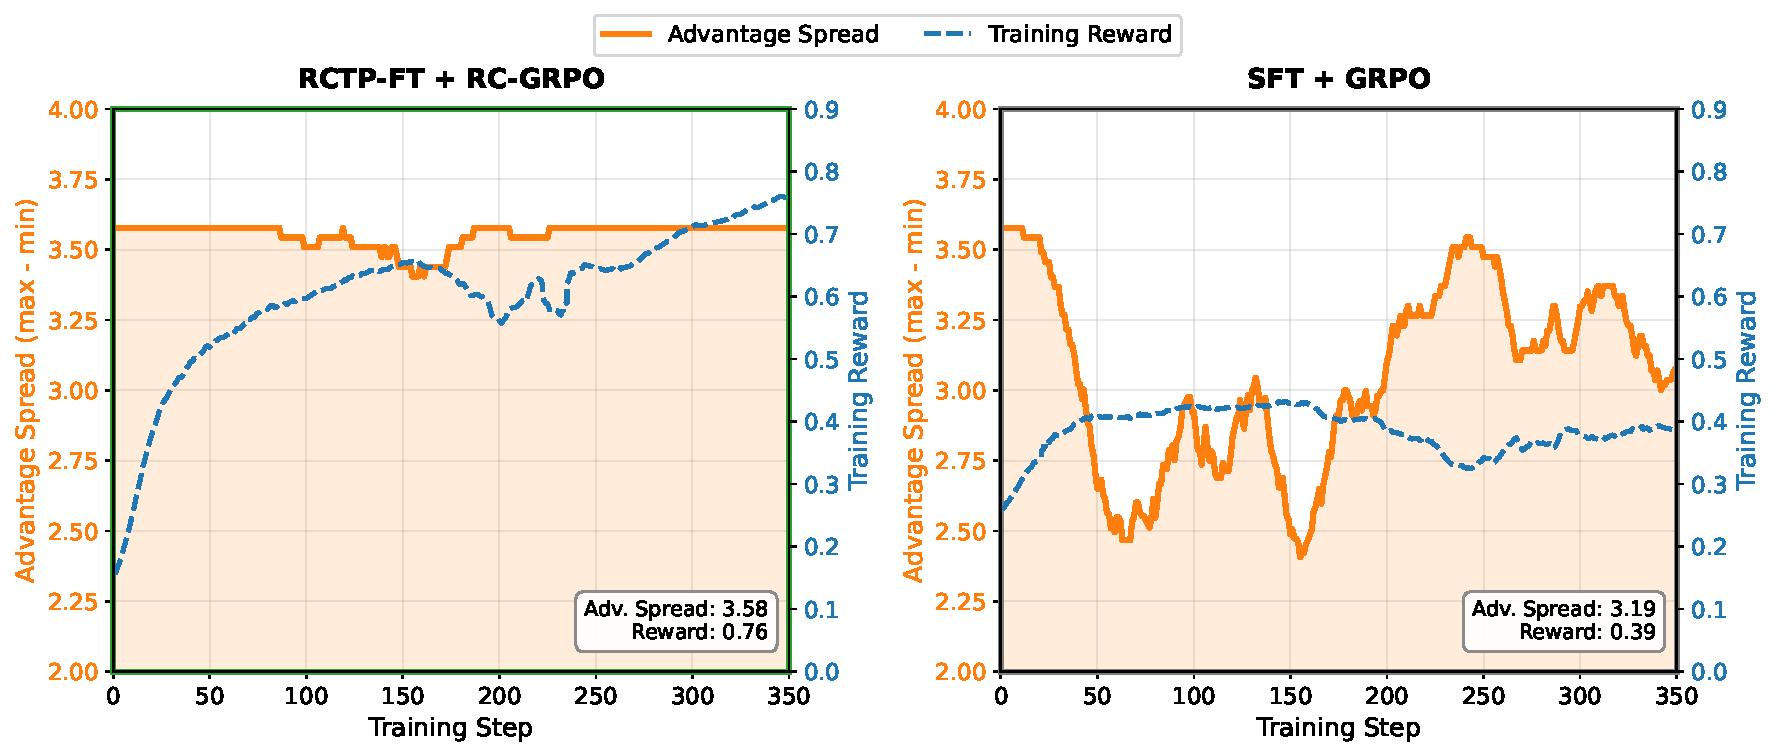
\includegraphics[width=\textwidth]{q3_advantage_spread.pdf}
  \caption{Training dynamics for Qwen2.5-7B on BFCLv4. We plot a proxy for within-group diversity (the gap between the maximum and minimum advantage within each sampled group) together with the training reward over time.}
  \label{fig:q3_advspread}
\end{figure*}

Taken together, Table~\ref{tab:q3_entropy} and Fig.~\ref{fig:q3_advspread} show that higher entropy is not required to maintain within-group diversity under RC-GRPO.
In our best-performing setting (RCTP+RC), entropy decreases over training (0.079$\to$0.037), yet reward improves and the entropy--reward correlation is negative ($\rho=-0.15$).
Meanwhile, under standard GRPO from the same RCTP initialization (RCTP+GRPO), reward is strongly positively correlated with entropy ($\rho=+0.49$), suggesting that entropy-based knobs act as an indirect and brittle route to exploration when the policy becomes peaked.

\textbf{Q4: Can we conduct theoretical justifications to explain why RC-GRPO works?} \\
\label{q4}
So far, we have focused on empirical results. We now complement them with a simple theoretical analysis and connect it to the observed training dynamics, to better illustrate why RC-GRPO is stable.
Specifically, we first analyze when standard GRPO can suffer from weak/vanishing group-normalized advantages, and then explain how reward-conditioned sampling restores within-group reward variance.

\label{sec:theory}
We do not claim a complete theory of multi-turn agent training dynamics; rather, we propose a minimal variance-based explanation for a common failure mode of standard GRPO when initialized from a peaked policy (e.g., after strong SFT). The key observation is that the Stage~2 GRPO update is mediated by the group-normalized advantage
$A_j = (R(\tau_j)-\mu_g)/(\sigma_g+\epsilon_{\text{stab}})$.
When group rollouts receive identical rewards, we have $R(\tau_j)=\mu_g$ for all $j$, so the numerator $(R(\tau_j)-\mu_g)$ is exactly zero and therefore $A_j=0$ (regardless of $\sigma_g$ and $\epsilon_{\text{stab}}$). In this case, the advantage-weighted update vanishes and learning stalls.
More generally, when rewards within a group are nearly identical, both $(R(\tau_j)-\mu_g)$ and $\sigma_g$ become small, yielding near-zero and/or noisy advantages (often effectively limited by the stability term $\epsilon_{\text{stab}}$), which again weakens the learning signal.
Proposition~\ref{prop:collapse} formalizes one sufficient condition under which such collapse can arise for standard (unconditioned) GRPO on peaked policies, while Proposition~\ref{prop:variance} shows how reward-conditioned sampling can prevent it by injecting between-mode reward variability within each group.

\begin{definition}[GRPO Advantage Collapse]
In GRPO with group size $G$, the advantage for trajectory $\tau_j$ is:
\begin{equation}
A_j = \frac{R(\tau_j) - \mu_g}{\sigma_g + \epsilon_{\text{stab}}}
\end{equation}
where $\mu_g$ and $\sigma_g$ are the within-group mean and standard deviation of $R(\tau)$. The advantage \emph{collapses} when $\sigma_g \to 0$, causing $A_j \to 0$ for all $j$ regardless of actual rewards.
\end{definition}

\begin{proposition}[Vanishing Gradient in Peaked Policies]
\label{prop:collapse}
Let $\pi_{\text{ref}}$ be trained on optimal demonstrations. Suppose that for each step $t$ (and history $h_t$ on the optimal trajectory), the SFT objective achieves a small per-step cross-entropy/KL to the optimal Dirac policy $\pi^*(\cdot|h_t)$:
\begin{equation}
    D_{\text{KL}}(\pi^*(\cdot|h_t)\,\|\,\pi_{\text{ref}}(\cdot|h_t)) \le \epsilon_{\text{sft}} .
\end{equation}
Then for a group of $G$ independent trajectories $\{\tau_1, \dots, \tau_G\}$ sampled from $\pi_{\text{ref}}$, the probability that all trajectories match the optimal trajectory $\tau^*$ satisfies
\begin{equation}
P(\tau_1 = \tau_2 = \cdots = \tau_G = \tau^*) \;\ge\; e^{-GT\epsilon_{\text{sft}}} \;\ge\; 1 - GT\epsilon_{\text{sft}}.
\end{equation}
On the event $\{\tau_1 = \cdots = \tau_G = \tau^*\}$, the within-group rewards are identical, so $\sigma_g = 0$ and $A_j = 0$ for all $j$. More generally, when $\pi_{\text{ref}}$ is sufficiently peaked so that rollouts within a group induce nearly identical rewards, we have $\sigma_g \ll \epsilon_{\text{stab}}$ and the normalized advantages are dominated by $\epsilon_{\text{stab}}$, making the effective learning signal negligible.
\end{proposition}

\begin{proof}[Proof Sketch]
Standard SFT on optimal-only data $\mathcal{D}_{\text{opt}}$ minimizes the negative log-likelihood of the optimal action, which can be written as $D_{\text{KL}}(\pi^* \| \pi_{\text{ref}})$ when $\pi^*$ is a Dirac measure on the optimal action. If $D_{\text{KL}}(\pi^*(\cdot|h_t)\,\|\,\pi_{\text{ref}}(\cdot|h_t)) \le \epsilon_{\text{sft}}$, then $-\log \pi_{\text{ref}}(a_t^*|h_t) \le \epsilon_{\text{sft}}$, hence $\pi_{\text{ref}}(a_t^*|h_t) \ge e^{-\epsilon_{\text{sft}}} \ge 1-\epsilon_{\text{sft}}$. Over $T$ steps, $P(\tau=\tau^*) \ge e^{-T\epsilon_{\text{sft}}} \ge 1-T\epsilon_{\text{sft}}$, and for $G$ independent samples, $P(\tau_1=\cdots=\tau_G=\tau^*) \ge e^{-GT\epsilon_{\text{sft}}} \ge 1-GT\epsilon_{\text{sft}}$. When trajectories are identical, $R(\tau_1)=\cdots=R(\tau_G)$ so $\sigma_g=0$ and all advantages collapse (hence the advantage-weighted policy-gradient term is zero). See Appendix~\ref{app:proofs} for the full proof.
\end{proof}

The key insight of RC-GRPO is to \emph{inject variance through conditioning} via the reward token $r \in \mathcal{R}$:

\begin{proposition}[Variance Guarantee via Reward Conditioning]
\label{prop:variance}
In RC-GRPO, each trajectory $\tau_j$ is conditioned on token $r_j \sim P_{\text{sample}}(r)$. If $\pi_{\text{ref}}$ learns distinct modes such that $|\mathbb{E}[R(\tau)|r_i] - \mathbb{E}[R(\tau)|r_j]| \geq \epsilon$ for $r_i \neq r_j$, then the within-group variance is lower-bounded:
\begin{equation}
\mathbb{E}\left[\sigma_g^2\right] \geq \kappa \epsilon^2
\end{equation}
where $\sigma_g^2 = \frac{1}{G}\sum_{j=1}^G (R(\tau_j)-\mu_g)^2$ is the (biased) within-group second central moment and $\kappa > 0$ depends on $P_{\text{sample}}(r)$ and $G$. In particular, with $p$ defined as in Eq.~\ref{eq:sampling}, one may take $\kappa=\frac{G-1}{G}p(1-p)$.
\end{proposition}

\begin{proof}[Proof Sketch]
By the law of total variance, $\text{Var}(R(\tau)) \ge \text{Var}_{r}(\mathbb{E}[R(\tau)|r])$. If the conditional means are separated by at least $\epsilon$, then $\text{Var}(R(\tau))\ge p(1-p)\epsilon^2$. Since $\sigma_g^2$ is the group second central moment over $G$ i.i.d.\ draws, $\mathbb{E}[\sigma_g^2]=\frac{G-1}{G}\text{Var}(R(\tau)) \ge \frac{G-1}{G}p(1-p)\epsilon^2$. See Appendix~\ref{app:proofs} for details.
\end{proof}

\begin{remark}[Convergence Implication]
\label{rem:convergence}
The expected variance lower bound $\mathbb{E}[\sigma_g^2] \geq \kappa\epsilon^2$ has direct implications for convergence speed. The signal-to-noise ratio of the GRPO gradient estimator depends on the typical scale of $\sigma_g$; by enforcing between-mode variability through $r$ and thereby preventing collapse of $\sigma_g$ in expectation, RC-GRPO maintains informative group-relative advantages throughout training. This contrasts with standard GRPO on peaked SFT models, where groups concentrate on a single trajectory and $\sigma_g$ collapses.
\end{remark}

In combination, Proposition~\ref{prop:collapse} and Proposition~\ref{prop:variance} explain why RC-GRPO avoids within-group variance collapse in practice. To empirically validate these theoretical claims, we analyze training dynamics in the late phase (the last 70 training steps) across four Qwen2.5-7B runs. Guided by Proposition~\ref{prop:collapse} and Proposition~\ref{prop:variance}, we operationalize within-group diversity using the \emph{advantage spread}---the difference between the maximum and minimum group-normalized advantage within each sampled group---as a direct proxy for how much signal the group normalization provides.

\begin{table}[t]
\centering
\caption{Late-phase training dynamics (last 70 training steps). RC-GRPO maintains high within-group diversity while keeping policy entropy low, consistent with the variance-guarantee mechanism.}
\label{tab:q4_dynamics}
\scriptsize
\setlength{\tabcolsep}{2pt}
\renewcommand{\arraystretch}{1.05}
\begin{tabular*}{\columnwidth}{@{\extracolsep{\fill}}lcccc}
\toprule
\textbf{Method} & \textbf{Spread} & \textbf{KL} & \textbf{$\|g\|$} & \textbf{$H$} \\
\midrule
\rowcolor{blue!10}
RCTP+RC (Ours) & \textbf{3.58} & 0.0010 & 2.7 & \textbf{0.037} \\
RCTP+GRPO & 3.46 & 0.0004 & 2.5 & 0.066 \\
SFT+GRPO & 3.22 & 0.0040 & 6.5 & 0.216 \\
SFT+RC & 3.51 & 0.0033 & 14.2 & 0.317 \\
\bottomrule
\end{tabular*}
\vspace{0.2em}

\footnotesize{Spread: max--min advantage within a sampled group; $\|g\|$: gradient norm; $H$: entropy.}
\end{table}

Table~\ref{tab:q4_dynamics} supports the variance-guarantee interpretation. Our method achieves the largest advantage spread (3.58) while maintaining the lowest entropy (0.037), indicating that within-group diversity is preserved without relying on increased policy randomness. In contrast, SFT + GRPO exhibits substantially higher entropy yet lower advantage spread, suggesting that entropy-based exploration alone is insufficient to reliably restore the within-group variability needed for informative group-normalized advantages.
Across all runs, gradient norms remain non-zero, but the combination of high spread and low entropy in RC-GRPO is most consistent with the intended between-mode separation induced by reward conditioning.

\section{Conclusion}
We introduced RC-GRPO, a two-stage pipeline (RCTP finetuning + reward-conditioned GRPO) for multi-turn tool calling that mitigates variance collapse in group-normalized policy optimization by making within-group diversity a controlled variable. Empirically, RC-GRPO delivers consistent gains on BFCLv4 for both Qwen2.5-7B and LLaMA-3.1-8B, with particularly large improvements when combined with the RCTP initialization. Our analysis suggests these gains are explained by more informative group-relative advantages (and non-vanishing updates) rather than simply increasing policy randomness. Theoretically, we provide a variance-based perspective that clarifies when standard GRPO can degenerate under peaked SFT policies and why reward-conditioned sampling prevents collapse. We hope this framing helps bridge controllable generation and group-based RL for training more reliable multi-turn tool-using agents.

\section*{Impact Statement}
This paper presents work whose goal is to advance the field of machine learning by improving the stability of reinforcement-learning optimization for multi-turn tool-calling agents. More reliable tool use can support beneficial applications such as automating routine digital tasks and enabling more capable assistants; at the same time, like other tool-using LLM systems, such capabilities may have dual-use implications if deployed without appropriate operational safeguards (e.g., access controls and monitoring). We expect the primary societal consequence of this work to be enabling further research on robust agent training and evaluation, rather than introducing fundamentally new deployment risks beyond those already associated with tool-enabled language models.


% \section{Electronic Submission}
% 
% Submission to ICML 2026 will be entirely electronic, via a web site
% (not email). Information about the submission process and \LaTeX\ templates
% are available on the conference web site at:
% \begin{center}
%   \texttt{http://icml.cc/}
% \end{center}
% 
% The guidelines below will be enforced for initial submissions and
% camera-ready copies. Here is a brief summary:
% \begin{itemize}
%   \item Submissions must be in PDF\@.
%   \item If your paper has appendices, submit the appendix together with the
%         main body and the references \textbf{as a single file}. Reviewers will not
%         look for appendices as a separate PDF file. So if you submit such an extra
%         file, reviewers will very likely miss it.
%   \item Page limit: The main body of the paper has to be fitted to 8 pages,
%         excluding references and appendices; the space for the latter two is not
%         limited in pages, but the total file size may not exceed 10MB. For the
%         final version of the paper, authors can add one extra page to the main
%         body.
%   \item \textbf{Do not include author information or acknowledgements} in your
%         initial submission.
%   \item Your paper should be in \textbf{10 point Times font}.
%   \item Make sure your PDF file only uses Type-1 fonts.
%   \item Place figure captions \emph{under} the figure (and omit titles from
%         inside the graphic file itself). Place table captions \emph{over} the
%         table.
%   \item References must include page numbers whenever possible and be as
%         complete as possible. Place multiple citations in chronological order.
%   \item Do not alter the style template; in particular, do not compress the
%         paper format by reducing the vertical spaces.
%   \item Keep your abstract brief and self-contained, one paragraph and roughly
%         4--6 sentences. Gross violations will require correction at the
%         camera-ready phase. The title should have content words capitalized.
% \end{itemize}
% 
% \subsection{Submitting Papers}
% 
% \textbf{Anonymous Submission:} ICML uses double-blind review: no identifying
% author information may appear on the title page or in the paper
% itself. \cref{author info} gives further details.
% 
% \medskip
% 
% Authors must provide their manuscripts in \textbf{PDF} format.
% Furthermore, please make sure that files contain only embedded Type-1 fonts
% (e.g.,~using the program \texttt{pdffonts} in linux or using
% File/DocumentProperties/Fonts in Acrobat). Other fonts (like Type-3)
% might come from graphics files imported into the document.
% 
% Authors using \textbf{Word} must convert their document to PDF\@. Most
% of the latest versions of Word have the facility to do this
% automatically. Submissions will not be accepted in Word format or any
% format other than PDF\@. Really. We're not joking. Don't send Word.
% 
% Those who use \textbf{\LaTeX} should avoid including Type-3 fonts.
% Those using \texttt{latex} and \texttt{dvips} may need the following
% two commands:
% 
% {\footnotesize
% \begin{verbatim}
% dvips -Ppdf -tletter -G0 -o paper.ps paper.dvi
% ps2pdf paper.ps
% \end{verbatim}}
% It is a zero following the ``-G'', which tells dvips to use
% the config.pdf file. Newer \TeX\ distributions don't always need this
% option.
% 
% Using \texttt{pdflatex} rather than \texttt{latex}, often gives better
% results. This program avoids the Type-3 font problem, and supports more
% advanced features in the \texttt{microtype} package.
% 
% \textbf{Graphics files} should be a reasonable size, and included from
% an appropriate format. Use vector formats (.eps/.pdf) for plots,
% lossless bitmap formats (.png) for raster graphics with sharp lines, and
% jpeg for photo-like images.
% 
% The style file uses the \texttt{hyperref} package to make clickable
% links in documents. If this causes problems for you, add
% \texttt{nohyperref} as one of the options to the \texttt{icml2026}
% usepackage statement.
% 
% \subsection{Submitting Final Camera-Ready Copy}
% 
% The final versions of papers accepted for publication should follow the
% same format and naming convention as initial submissions, except that
% author information (names and affiliations) should be given. See
% \cref{final author} for formatting instructions.
% 
% The footnote, ``Preliminary work. Under review by the International
% Conference on Machine Learning (ICML). Do not distribute.'' must be
% modified to ``\textit{Proceedings of the
%   $\mathit{43}^{rd}$ International Conference on Machine Learning},
% Seoul, South Korea, PMLR 306, 2026.
% Copyright 2026 by the author(s).''
% 
% For those using the \textbf{\LaTeX} style file, this change (and others) is
% handled automatically by simply changing
% $\mathtt{\backslash usepackage\{icml2026\}}$ to
% $$\mathtt{\backslash usepackage[accepted]\{icml2026\}}$$
% Authors using \textbf{Word} must edit the
% footnote on the first page of the document themselves.
% 
% Camera-ready copies should have the title of the paper as running head
% on each page except the first one. The running title consists of a
% single line centered above a horizontal rule which is $1$~point thick.
% The running head should be centered, bold and in $9$~point type. The
% rule should be $10$~points above the main text. For those using the
% \textbf{\LaTeX} style file, the original title is automatically set as running
% head using the \texttt{fancyhdr} package which is included in the ICML
% 2026 style file package. In case that the original title exceeds the
% size restrictions, a shorter form can be supplied by using
% 
% \verb|\icmltitlerunning{...}|
% 
% just before $\mathtt{\backslash begin\{document\}}$.
% Authors using \textbf{Word} must edit the header of the document themselves.
% 
% \section{Format of the Paper}
% 
% All submissions must follow the specified format.
% 
% \subsection{Dimensions}
% 
% The text of the paper should be formatted in two columns, with an
% overall width of 6.75~inches, height of 9.0~inches, and 0.25~inches
% between the columns. The left margin should be 0.75~inches and the top
% margin 1.0~inch (2.54~cm). The right and bottom margins will depend on
% whether you print on US letter or A4 paper, but all final versions
% must be produced for US letter size.
% Do not write anything on the margins.
% 
% The paper body should be set in 10~point type with a vertical spacing
% of 11~points. Please use Times typeface throughout the text.
% 
% \subsection{Title}
% 
% The paper title should be set in 14~point bold type and centered
% between two horizontal rules that are 1~point thick, with 1.0~inch
% between the top rule and the top edge of the page. Capitalize the
% first letter of content words and put the rest of the title in lower
% case.
% You can use TeX math in the title (we suggest sparingly),
% but no custom macros, images, or other TeX commands.
% Please make sure that accents, special characters, etc., are entered using
% TeX commands and not using non-English characters.
% 
% \subsection{Author Information for Submission}
% \label{author info}
% 
% ICML uses double-blind review, so author information must not appear. If
% you are using \LaTeX\/ and the \texttt{icml2026.sty} file, use
% \verb+\icmlauthor{...}+ to specify authors and \verb+\icmlaffiliation{...}+
% to specify affiliations. (Read the TeX code used to produce this document for
% an example usage.) The author information will not be printed unless
% \texttt{accepted} is passed as an argument to the style file. Submissions that
% include the author information will not be reviewed.
% 
% \subsubsection{Self-Citations}
% 
% If you are citing published papers for which you are an author, refer
% to yourself in the third person. In particular, do not use phrases
% that reveal your identity (e.g., ``in previous work \cite{langley00}, we
% have shown \ldots'').
% 
% Do not anonymize citations in the reference section. The only exception are manuscripts that are
% not yet published (e.g., under submission). If you choose to refer to
% such unpublished manuscripts \cite{anonymous}, anonymized copies have
% to be submitted
% as Supplementary Material via OpenReview\@. However, keep in mind that an ICML
% paper should be self contained and should contain sufficient detail
% for the reviewers to evaluate the work. In particular, reviewers are
% not required to look at the Supplementary Material when writing their
% review (they are not required to look at more than the first $8$ pages of the submitted document).
% 
% \subsubsection{Camera-Ready Author Information}
% \label{final author}
% 
% If a paper is accepted, a final camera-ready copy must be prepared.
% %
% For camera-ready papers, author information should start 0.3~inches below the
% bottom rule surrounding the title. The authors' names should appear in 10~point
% bold type, in a row, separated by white space, and centered. Author names should
% not be broken across lines. Unbolded superscripted numbers, starting 1, should
% be used to refer to affiliations.
% 
% Affiliations should be numbered in the order of appearance. A single footnote
% block of text should be used to list all the affiliations. (Academic
% affiliations should list Department, University, City, State/Region, Country.
% Similarly for industrial affiliations.)
% 
% Each distinct affiliations should be listed once. If an author has multiple
% affiliations, multiple superscripts should be placed after the name, separated
% by thin spaces. If the authors would like to highlight equal contribution by
% multiple first authors, those authors should have an asterisk placed after their
% name in superscript, and the term ``\textsuperscript{*}Equal contribution"
% should be placed in the footnote block ahead of the list of affiliations. A
% list of corresponding authors and their emails (in the format Full Name
% \textless{}email@domain.com\textgreater{}) can follow the list of affiliations.
% Ideally only one or two names should be listed.
% 
% A sample file with author names is included in the ICML2026 style file
% package. Turn on the \texttt{[accepted]} option to the stylefile to
% see the names rendered. All of the guidelines above are implemented
% by the \LaTeX\ style file.
% 
% \subsection{Abstract}
% 
% The paper abstract should begin in the left column, 0.4~inches below the final
% address. The heading `Abstract' should be centered, bold, and in 11~point type.
% The abstract body should use 10~point type, with a vertical spacing of
% 11~points, and should be indented 0.25~inches more than normal on left-hand and
% right-hand margins. Insert 0.4~inches of blank space after the body. Keep your
% abstract brief and self-contained, limiting it to one paragraph and roughly 4--6
% sentences. Gross violations will require correction at the camera-ready phase.
% 
% \subsection{Partitioning the Text}
% 
% You should organize your paper into sections and paragraphs to help readers
% place a structure on the material and understand its contributions.
% 
% \subsubsection{Sections and Subsections}
% 
% Section headings should be numbered, flush left, and set in 11~pt bold type
% with the content words capitalized. Leave 0.25~inches of space before the
% heading and 0.15~inches after the heading.
% 
% Similarly, subsection headings should be numbered, flush left, and set in 10~pt
% bold type with the content words capitalized. Leave
% 0.2~inches of space before the heading and 0.13~inches afterward.
% 
% Finally, subsubsection headings should be numbered, flush left, and set in
% 10~pt small caps with the content words capitalized. Leave
% 0.18~inches of space before the heading and 0.1~inches after the heading.
% 
% Please use no more than three levels of headings.
% 
% \subsubsection{Paragraphs and Footnotes}
% 
% Within each section or subsection, you should further partition the paper into
% paragraphs. Do not indent the first line of a given paragraph, but insert a
% blank line between succeeding ones.
% 
% You can use footnotes\footnote{Footnotes should be complete sentences.}
% to provide readers with additional information about a topic without
% interrupting the flow of the paper. Indicate footnotes with a number in the
% text where the point is most relevant. Place the footnote in 9~point type at
% the bottom of the column in which it appears. Precede the first footnote in a
% column with a horizontal rule of 0.8~inches.\footnote{Multiple footnotes can
%   appear in each column, in the same order as they appear in the text,
%   but spread them across columns and pages if possible.}
% 
% \begin{figure}[ht]
%   \vskip 0.2in
%   \begin{center}
%     \centerline{
\includegraphics[width=\columnwidth]{icml_numpapers}}
%     \caption{
%       Historical locations and number of accepted papers for International
%       Machine Learning Conferences (ICML 1993 -- ICML 2008) and International
%       Workshops on Machine Learning (ML 1988 -- ML 1992). At the time this
%       figure was produced, the number of accepted papers for ICML 2008 was
%       unknown and instead estimated.
%     }
%     \label{icml-historical}
%   \end{center}
% \end{figure}
% 
% \subsection{Figures}
% 
% You may want to include figures in the paper to illustrate your approach and
% results. Such artwork should be centered, legible, and separated from the text.
% Lines should be dark and at least 0.5~points thick for purposes of
% reproduction, and text should not appear on a gray background.
% 
% Label all distinct components of each figure. If the figure takes the form of a
% graph, then give a name for each axis and include a legend that briefly
% describes each curve. Do not include a title inside the figure; instead, the
% caption should serve this function.
% 
% Number figures sequentially, placing the figure number and caption \emph{after}
% the graphics, with at least 0.1~inches of space before the caption and
% 0.1~inches after it, as in \cref{icml-historical}. The figure caption should be
% set in 9~point type and centered unless it runs two or more lines, in which
% case it should be flush left. You may float figures to the top or bottom of a
% column, and you may set wide figures across both columns (use the environment
% \texttt{figure*} in \LaTeX). Always place two-column figures at the top or
% bottom of the page.
% 
% \subsection{Algorithms}
% 
% If you are using \LaTeX, please use the ``algorithm'' and ``algorithmic''
% environments to format pseudocode. These require the corresponding stylefiles,
% algorithm.sty and algorithmic.sty, which are supplied with this package.
% \cref{alg:example} shows an example.
% 
% \begin{algorithm}[tb]
%   \caption{Bubble Sort}
%   \label{alg:example}
%   \begin{algorithmic}
%     \STATE {\bfseries Input:} data $x_i$, size $m$
%     \REPEAT
%     \STATE Initialize $noChange = true$.
%     \FOR{$i=1$ {\bfseries to} $m-1$}
%     \IF{$x_i > x_{i+1}$}
%     \STATE Swap $x_i$ and $x_{i+1}$
%     \STATE $noChange = false$
%     \ENDIF
%     \ENDFOR
%     \UNTIL{$noChange$ is $true$}
%   \end{algorithmic}
% \end{algorithm}
% 
% 
% \subsection{Tables}
% 
% You may also want to include tables that summarize material. Like figures,
% these should be centered, legible, and numbered consecutively. However, place
% the title \emph{above} the table with at least 0.1~inches of space before the
% title and the same after it, as in \cref{sample-table}. The table title should
% be set in 9~point type and centered unless it runs two or more lines, in which
% case it should be flush left.
% 
% % Note use of \abovespace and \belowspace to get reasonable spacing
% % above and below tabular lines.
% 
% \begin{table}[t]
%   \caption{Classification accuracies for naive Bayes and flexible
%     Bayes on various data sets.}
%   \label{sample-table}
%   \begin{center}
%     \begin{small}
%       \begin{sc}
%         \begin{tabular}{lcccr}
%           \toprule
%           Data set  & Naive         & Flexible      & Better?  \\
%           \midrule
%           Breast    & 95.9$\pm$ 0.2 & 96.7$\pm$ 0.2 & $\surd$  \\
%           Cleveland & 83.3$\pm$ 0.6 & 80.0$\pm$ 0.6 & $\times$ \\
%           Glass2    & 61.9$\pm$ 1.4 & 83.8$\pm$ 0.7 & $\surd$  \\
%           Credit    & 74.8$\pm$ 0.5 & 78.3$\pm$ 0.6 &          \\
%           Horse     & 73.3$\pm$ 0.9 & 69.7$\pm$ 1.0 & $\times$ \\
%           Meta      & 67.1$\pm$ 0.6 & 76.5$\pm$ 0.5 & $\surd$  \\
%           Pima      & 75.1$\pm$ 0.6 & 73.9$\pm$ 0.5 &          \\
%           Vehicle   & 44.9$\pm$ 0.6 & 61.5$\pm$ 0.4 & $\surd$  \\
%           \bottomrule
%         \end{tabular}
%       \end{sc}
%     \end{small}
%   \end{center}
%   \vskip -0.1in
% \end{table}
% 
% Tables contain textual material, whereas figures contain graphical material.
% Specify the contents of each row and column in the table's topmost row. Again,
% you may float tables to a column's top or bottom, and set wide tables across
% both columns. Place two-column tables at the top or bottom of the page.
% 
% \subsection{Theorems and Such}
% The preferred way is to number definitions, propositions, lemmas, etc.
% consecutively, within sections, as shown below.
% \begin{definition}
%   \label{def:inj}
%   A function $f:X \to Y$ is injective if for any $x,y\in X$ different, $f(x)\ne
%     f(y)$.
% \end{definition}
% Using \cref{def:inj} we immediate get the following result:
% \begin{proposition}
%   If $f$ is injective mapping a set $X$ to another set $Y$,
%   the cardinality of $Y$ is at least as large as that of $X$
% \end{proposition}
% \begin{proof}
%   Left as an exercise to the reader.
% \end{proof}
% \cref{lem:usefullemma} stated next will prove to be useful.
% \begin{lemma}
%   \label{lem:usefullemma}
%   For any $f:X \to Y$ and $g:Y\to Z$ injective functions, $f \circ g$ is
%   injective.
% \end{lemma}
% \begin{theorem}
%   \label{thm:bigtheorem}
%   If $f:X\to Y$ is bijective, the cardinality of $X$ and $Y$ are the same.
% \end{theorem}
% An easy corollary of \cref{thm:bigtheorem} is the following:
% \begin{corollary}
%   If $f:X\to Y$ is bijective,
%   the cardinality of $X$ is at least as large as that of $Y$.
% \end{corollary}
% \begin{assumption}
%   The set $X$ is finite.
%   \label{ass:xfinite}
% \end{assumption}
% \begin{remark}
%   According to some, it is only the finite case (cf. \cref{ass:xfinite}) that
%   is interesting.
% \end{remark}
% %restatable
% 
% \subsection{Citations and References}
% 
% Please use APA reference format regardless of your formatter or word processor.
% If you rely on the \LaTeX\/ bibliographic facility, use \texttt{natbib.sty} and
% \texttt{icml2026.bst} included in the style-file package to obtain this format.
% 
% Citations within the text should include the authors' last names and year. If
% the authors' names are included in the sentence, place only the year in
% parentheses, for example when referencing Arthur Samuel's pioneering work
% \yrcite{Samuel59}. Otherwise place the entire reference in parentheses with the
% authors and year separated by a comma \cite{Samuel59}. List multiple references
% separated by semicolons \cite{kearns89,Samuel59,mitchell80}. Use the `et~al.'
% construct only for citations with three or more authors or after listing all
% authors to a publication in an earlier reference \cite{MachineLearningI}.
% 
% Authors should cite their own work in the third person in the initial version
% of their paper submitted for blind review. Please refer to \cref{author info}
% for detailed instructions on how to cite your own papers.
% 
% Use an unnumbered first-level section heading for the references, and use a
% hanging indent style, with the first line of the reference flush against the
% left margin and subsequent lines indented by 10 points. The references at the
% end of this document give examples for journal articles \cite{Samuel59},
% conference publications \cite{langley00}, book chapters \cite{Newell81}, books
% \cite{DudaHart2nd}, edited volumes \cite{MachineLearningI}, technical reports
% \cite{mitchell80}, and dissertations \cite{kearns89}.
% 
% Alphabetize references by the surnames of the first authors, with single author
% entries preceding multiple author entries. Order references for the same
% authors by year of publication, with the earliest first. Make sure that each
% reference includes all relevant information (e.g., page numbers).
% 
% Please put some effort into making references complete, presentable, and
% consistent, e.g. use the actual current name of authors. If using bibtex,
% please protect capital letters of names and abbreviations in titles, for
% example, use \{B\}ayesian or \{L\}ipschitz in your .bib file.
% 
% \section*{Accessibility}
% 
% Authors are kindly asked to make their submissions as accessible as possible
% for everyone including people with disabilities and sensory or neurological
% differences. Tips of how to achieve this and what to pay attention to will be
% provided on the conference website \url{http://icml.cc/}.
% 
% \section*{Software and Data}
% 
% If a paper is accepted, we strongly encourage the publication of software and
% data with the camera-ready version of the paper whenever appropriate. This can
% be done by including a URL in the camera-ready copy. However, \textbf{do not}
% include URLs that reveal your institution or identity in your submission for
% review. Instead, provide an anonymous URL or upload the material as
% ``Supplementary Material'' into the OpenReview reviewing system. Note that
% reviewers are not required to look at this material when writing their review.
% 
% % Acknowledgements should only appear in the accepted version.
% \section*{Impact Statement}
% 
% Authors are \textbf{required} to include a statement of the potential broader
% impact of their work, including its ethical aspects and future societal
% consequences. This statement should be in an unnumbered section at the end of
% the paper (co-located with Acknowledgements -- the two may appear in either
% order, but both must be before References), and does not count toward the paper
% page limit. In many cases, where the ethical impacts and expected societal
% implications are those that are well established when advancing the field of
% Machine Learning, substantial discussion is not required, and a simple
% statement such as the following will suffice:
% 
% ``This paper presents work whose goal is to advance the field of Machine
% Learning. There are many potential societal consequences of our work, none
% which we feel must be specifically highlighted here.''
% 
% The above statement can be used verbatim in such cases, but we encourage
% authors to think about whether there is content which does warrant further
% discussion, as this statement will be apparent if the paper is later flagged
% for ethics review.

% In the unusual situation where you want a paper to appear in the
% references without citing it in the main text, use \nocite

\bibliography{example_paper}
\bibliographystyle{icml2026}

%%%%%%%%%%%%%%%%%%%%%%%%%%%%%%%%%%%%%%%%%%%%%%%%%%%%%%%%%%%%%%%%%%%%%%%%%%%%%%%
%%%%%%%%%%%%%%%%%%%%%%%%%%%%%%%%%%%%%%%%%%%%%%%%%%%%%%%%%%%%%%%%%%%%%%%%%%%%%%%
% APPENDIX
%%%%%%%%%%%%%%%%%%%%%%%%%%%%%%%%%%%%%%%%%%%%%%%%%%%%%%%%%%%%%%%%%%%%%%%%%%%%%%%
%%%%%%%%%%%%%%%%%%%%%%%%%%%%%%%%%%%%%%%%%%%%%%%%%%%%%%%%%%%%%%%%%%%%%%%%%%%%%%%
\newpage
\appendix
\onecolumn
\section{Theoretical Proofs}
\label{app:proofs}

This appendix provides formal proofs for the theoretical results presented in the main text.

\subsection{Proof of Proposition~\ref{prop:collapse}}

We first state the definitions and lemmas used in the proof.

\begin{definition}[Probability Space]
Let $(\mathcal{A}, \Sigma, P)$ be a discrete probability space over the set of actions $\mathcal{A}$. Let $\pi_{\text{ref}}$ and $\pi^*$ be probability measures on this space.
\end{definition}

\begin{lemma}[KL-Probability Bound]
\label{lem:kl_bound}
Let $\pi^*$ be a Dirac measure concentrated at $a^*$, i.e., $\pi^*(a^*) = 1$. If $D_{\text{KL}}(\pi^* \| \pi) \le \epsilon$, then:
\begin{equation}
\pi(a^*) \ge e^{-\epsilon} \ge 1 - \epsilon
\end{equation}
\end{lemma}

\begin{proof}[Proof of Lemma~\ref{lem:kl_bound}]
Since $\pi^*$ is a Dirac measure:
\begin{equation}
D_{\text{KL}}(\pi^* \| \pi) = \sum_{a} \pi^*(a) \log \frac{\pi^*(a)}{\pi(a)} = 1 \cdot \log \frac{1}{\pi(a^*)} = -\log \pi(a^*)
\end{equation}
Given $D_{\text{KL}}(\pi^* \| \pi) \le \epsilon$, we have $-\log \pi(a^*) \le \epsilon \implies \pi(a^*) \ge e^{-\epsilon}$. Using the inequality $e^{-x} \ge 1-x$ for $x \ge 0$, we get $\pi(a^*) \ge 1 - \epsilon$.
\end{proof}

\begin{proof}[Proof of Proposition~\ref{prop:collapse}]
Fix an optimal trajectory $\tau^*=(h_1^*,a_1^*,\dots,h_T^*,a_T^*)$ and let $h_t^*$ denote the history on this optimal trajectory at step $t$. Under the proposition assumption,
\begin{equation}
D_{\mathrm{KL}}\!\left(\pi^*(\cdot\mid h_t^*)\,\middle\|\,\pi_{\mathrm{ref}}(\cdot\mid h_t^*)\right)\le \epsilon_{\text{sft}}
\quad\Rightarrow\quad
\pi_{\mathrm{ref}}(a_t^*\mid h_t^*) \ge e^{-\epsilon_{\text{sft}}}
\end{equation}
by Lemma~\ref{lem:kl_bound}. Therefore the probability that a single rollout from $\pi_{\mathrm{ref}}$ exactly follows the optimal trajectory is
\begin{equation}
P(\tau=\tau^*) \;=\; \prod_{t=1}^{T}\pi_{\mathrm{ref}}(a_t^*\mid h_t^*) \;\ge\; e^{-T\epsilon_{\text{sft}}} \;\ge\; 1-T\epsilon_{\text{sft}},
\end{equation}
where we used $\prod_{t=1}^T e^{-\epsilon_{\text{sft}}}=e^{-T\epsilon_{\text{sft}}}$ and the inequality $e^{-x}\ge 1-x$ for $x\ge 0$.

Now sample $G$ independent trajectories $\tau_1,\dots,\tau_G \overset{\text{i.i.d.}}{\sim}\pi_{\mathrm{ref}}$. Then
\begin{equation}
P(\tau_1=\cdots=\tau_G=\tau^*) \;=\; P(\tau=\tau^*)^G \;\ge\; e^{-GT\epsilon_{\text{sft}}} \;\ge\; 1-GT\epsilon_{\text{sft}}.
\end{equation}

On the event $\{\tau_1=\cdots=\tau_G\}$, we have $R(\tau_1)=\cdots=R(\tau_G)$, hence $\sigma_g=0$ and $R(\tau_j)-\mu_g=0$ for every $j$. Therefore $A_j=\frac{R(\tau_j)-\mu_g}{\sigma_g+\epsilon_{\text{stab}}}=0$ for all $j$, and the advantage-weighted GRPO policy-gradient term for that group,
\begin{equation}
\frac{1}{G}\sum_{j=1}^G A_j \sum_{t=1}^{T}\nabla_\theta \log \pi_\theta(a_{t,j}\mid h_{t,j})
\end{equation}
is exactly zero.
\end{proof}

\subsection{Proof of Proposition~\ref{prop:variance}}

We first state the key lemmas used in this proof.

\begin{lemma}[Law of Total Variance]
\label{lem:total_variance}
For random variables $X$ and $Y$, the total variance of $X$ decomposes as:
\begin{equation}
\text{Var}(X) = \underbrace{\mathbb{E}_{Y}[\text{Var}(X|Y)]}_{\text{within-group variance}} + \underbrace{\text{Var}_{Y}(\mathbb{E}[X|Y])}_{\text{between-group variance}}
\end{equation}
Since the first term is non-negative, we have $\text{Var}(X) \ge \text{Var}_{Y}(\mathbb{E}[X|Y])$.
\end{lemma}

\begin{lemma}[Expected Group Second Central Moment]
\label{lem:expected_group_var}
Let $X_1,\dots,X_G$ be i.i.d.\ with finite variance $\text{Var}(X)$. Define $\bar{X}=\frac{1}{G}\sum_{j=1}^G X_j$ and $S_G^2=\frac{1}{G}\sum_{j=1}^G (X_j-\bar{X})^2$. Then
\begin{equation}
\mathbb{E}[S_G^2] = \frac{G-1}{G}\,\text{Var}(X).
\end{equation}
\end{lemma}

\begin{proof}
Using $S_G^2=\frac{1}{G}\sum_{j=1}^G X_j^2-\bar{X}^2$ and letting $\mu=\mathbb{E}[X]$, we have
\begin{equation}
\mathbb{E}[S_G^2] = \mathbb{E}[X^2] - \mathbb{E}[\bar{X}^2]
= \mathbb{E}[X^2] - \big(\text{Var}(\bar{X}) + (\mathbb{E}[\bar{X}])^2\big)
= (\text{Var}(X)+\mu^2) - \left(\frac{1}{G}\text{Var}(X)+\mu^2\right),
\end{equation}
which yields $\mathbb{E}[S_G^2]=\frac{G-1}{G}\text{Var}(X)$.
\end{proof}

\begin{proof}[Proof of Proposition~\ref{prop:variance}]
Let $r\in\{\texttt{high},\texttt{low}\}$ be sampled from $P_{\mathrm{sample}}$ with $p:=P_{\mathrm{sample}}(r=\texttt{high})\in(0,1)$. Let $\tau\sim \pi_{\mathrm{ref}}(\cdot\mid r)$ and define the bounded reward random variable $X:=R(\tau)\in[0,1]$. Let $\mu_h:=\mathbb{E}[X\mid r=\texttt{high}]$ and $\mu_l:=\mathbb{E}[X\mid r=\texttt{low}]$.

By Lemma~\ref{lem:total_variance} (law of total variance),
\begin{equation}
\text{Var}(X) \;\ge\; \text{Var}_{r}\!\big(\mathbb{E}[X\mid r]\big)
 \;=\; p(1-p)\,(\mu_h-\mu_l)^2.
\end{equation}
Under the proposition assumption $|\mu_h-\mu_l|\ge \epsilon$, we obtain
\begin{equation}
\text{Var}(X) \ge p(1-p)\,\epsilon^2.
\end{equation}

Now draw a GRPO group by sampling $G$ i.i.d.\ pairs $(r_j,\tau_j)$ with $r_j\sim P_{\mathrm{sample}}$ and $\tau_j\sim \pi_{\mathrm{ref}}(\cdot\mid r_j)$, and define $X_j:=R(\tau_j)$ and $\sigma_g^2:=\frac{1}{G}\sum_{j=1}^G (X_j-\bar{X})^2$ where $\bar{X}=\frac{1}{G}\sum_{j=1}^G X_j$. By Lemma~\ref{lem:expected_group_var},
\begin{equation}
\mathbb{E}[\sigma_g^2] = \frac{G-1}{G}\,\text{Var}(X)
\;\ge\; \frac{G-1}{G}\,p(1-p)\,\epsilon^2.
\end{equation}
Thus we can take $\kappa=\frac{G-1}{G}p(1-p)$.
\end{proof}

\section{The Details of the Dataset Formulations}
\label{app:dataset}

\subsection{Berkeley Function Calling Leaderboard (BFCLv4)}
The Berkeley Function Calling Leaderboard (BFCLv4) \cite{bfcl2024} is a comprehensive benchmark designed to evaluate the tool-calling capabilities of Large Language Models. It encompasses a wide variety of APIs (e.g., Java, JavaScript, Python) and diverse scenarios. Our work primarily focuses on the \textbf{multi-turn dataset} section, which is specifically designed to test an agent's ability to maintain context, handle state changes, and execute sequential tools to achieve a complex goal.

\textbf{Benchmark Statistics.}
The multi-turn subset consists of 200 high-quality, human-curated evaluation trajectories. Each trajectory involves multiple steps (typically 3-10 turns) where the agent must interact with a simulated environment. The primary domains include:
\begin{itemize}
    \item \textbf{GorillaFileSystem:} A simulated Linux file system supporting commands like \texttt{ls}, \texttt{cd}, \texttt{grep}, \texttt{find}, \texttt{mv}, etc.
    \item \textbf{TwitterAPI:} A mock social media API for posting tweets, replying, and managing followers.
    \item \textbf{MathAPI:} Utilities for statistical calculations (mean, standard deviation, logarithm).
    \item \textbf{TicketAPI:} A system for managing support tickets (create, resolve, query).
\end{itemize}

\subsubsection{Data Curation Pipeline}
\label{app:bfcl_curation}

We employ a systematic pipeline to construct aligned SFT, RCTP-FT, and RL datasets for BFCLv4 multi-turn evaluation. All datasets share the same ID-based train/test split (90\%/10\%) to ensure zero question overlap between training and evaluation.

\paragraph{Stage 1: SFT and RCTP-FT Data.}

\textit{Source.} We derive training data from two complementary sources. Since the RCTP-FT training dataset uses an exact 1:1 expert-to-failure ratio (800:800), we set $p=0.5$ in Eq.~\ref{eq:sampling}.
\begin{itemize}
    \item \textbf{Expert Trajectories (800):} Extracted from the official BFCLv4 ground truth (\texttt{possible\_answer/} files). These represent optimal execution paths verified by the benchmark maintainers across four multi-turn categories: \texttt{base}, \texttt{long\_context}, \texttt{miss\_func}, and \texttt{miss\_param} (200 samples each).
    \item \textbf{Failure Trajectories (800):} Collected via RL exploration rollouts using Qwen2.5-7B-Instruct. These capture diverse failure modes including incorrect tool selection, parameter errors, and premature termination.
\end{itemize}

\textit{Split.} We apply an ID-based split: 720 train / 80 test. This ensures that questions sharing the same numeric ID (which appear across multiple categories) are kept together in either train or test, preventing data leakage.

\textit{Format.} Both SFT and RCTP-FT datasets use OpenAI chat format with a combined task prompt (``Step 1: ... Step 2: ... Complete all the steps above using the available tools. Call done() when you have finished all tasks.''). The key distinction:
\begin{itemize}
    \item \textbf{SFT:} Expert trajectories only, no reward tokens.
    \item \textbf{RCTP-FT:} Both expert and failure trajectories, with reward token appended to the first user message: \texttt{[Reward Goal: <|high\_reward|>]} for success and \texttt{[Reward Goal: <|low\_reward|>]} for failure.
\end{itemize}

\textit{Statistics.} Table~\ref{tab:bfcl_stats} summarizes the curated data. The RCTP-FT dataset maintains an exact 50-50 balance between success and failure trajectories, which is essential for learning reward-conditioned generation.

\begin{table}[h]
\centering
\caption{SFT and RCTP-FT Dataset Statistics for BFCLv4}
\label{tab:bfcl_stats}
\small
\begin{tabular}{@{}lcccc@{}}
\toprule
\textbf{Dataset} & \textbf{Train} & \textbf{Test} & \textbf{Total} & \textbf{Success Rate} \\
\midrule
SFT & 720 & 80 & 800 & 100\% \\
\midrule
RCTP-FT (success) & 720 & 80 & 800 & 100\% \\
RCTP-FT (failure) & 720 & 80 & 800 & 0\% \\
\textbf{RCTP-FT Total} & \textbf{1,440} & \textbf{160} & \textbf{1,600} & \textbf{50\%} \\
\bottomrule
\end{tabular}
\end{table}

\paragraph{Stage 2: RL Data.}

\textit{Source.} For online RL, we use minimal task pointers that reference the original BFCLv4 questions. The BFCL environment adapter constructs the full system prompt and combined task prompt at runtime, enabling dynamic interaction with the simulated environment.

\textit{Split.} We use the same ID-based split as Stage 1: 720 train / 80 test. Table~\ref{tab:rl_split} shows the distribution across categories. The per-category counts are not exactly 180/20 because the split operates at the ID level first, and samples sharing an ID inherit that assignment.

\begin{table}[h]
\centering
\caption{RL Data Train/Test Split by Category}
\label{tab:rl_split}
\small
\begin{tabular}{@{}lccc@{}}
\toprule
\textbf{Category} & \textbf{Train} & \textbf{Test} & \textbf{Total} \\
\midrule
multi\_turn\_base & 182 & 18 & 200 \\
multi\_turn\_long\_context & 177 & 23 & 200 \\
multi\_turn\_miss\_func & 183 & 17 & 200 \\
multi\_turn\_miss\_param & 178 & 22 & 200 \\
\midrule
\textbf{Total} & \textbf{720} & \textbf{80} & \textbf{800} \\
\bottomrule
\end{tabular}
\end{table}

\textit{Format.} Each RL sample is a minimal task pointer:
\begin{verbatim}
{
  "conversations": [{"from": "human", "value": "[BFCL task: multi_turn_base_0]"}],
  "task_id": "multi_turn_base_0",
  "source_file": "BFCL_v4_multi_turn_base.json",
  "env_type": "bfcl"
}
\end{verbatim}

\paragraph{Format Alignment.}
All data phases enforce strict format alignment to ensure consistency across SFT, RCTP-FT, and RL:
\begin{enumerate}
    \item \textbf{Message Structure:} OpenAI chat format (\texttt{\{role, content, tool\_calls\}}).
    \item \textbf{Combined Task Prompt:} User instructions are merged into a single ``Step 1: ..., Step 2: ...'' format.
    \item \textbf{Schema Consistency:} All assistant messages include an explicit \texttt{tool\_calls} key (empty list if no calls).
\end{enumerate}

\subsubsection{Data Examples}
\label{app:examples}

We provide examples to illustrate the data formats used in each training stage.

\paragraph{Multi-Turn Trajectory Example.}
This example from \texttt{multi\_turn\_base\_1} demonstrates a task requiring file system manipulation. During SFT/RCTP-FT, the model observes multi-turn user queries as separate turns. During RL, the queries are merged into a single combined task prompt.

\begin{defaultbox}
\textbf{Task ID:} \texttt{multi\_turn\_base\_1} \\
\textbf{User Query 1:} ``I am alex. Check if the current directory is under my name and list all the visible and hidden contents in the current directory now, please.'' \\
\textbf{Agent Action 1:} \texttt{ls(a=True)} \\
\textbf{Observation 1:} \texttt{\{"status": "success"\}}

\textbf{User Query 2:} ``Go to workspace directory and move one of the 'log.txt' files into a new directory 'archive'.'' \\
\textbf{Agent Action 2:} \texttt{cd(folder="workspace")} \\
\textbf{Agent Action 3:} \texttt{mv(source="log.txt", destination="archive")}

\textbf{User Query 3:} ``Investigate within 'log.txt' for the occurrence of the keyword 'Error'.'' \\
\textbf{Agent Action 4:} \texttt{cd(folder="archive")} \\
\textbf{Agent Action 5:} \texttt{grep(file\_name="log.txt", pattern="Error")}
\end{defaultbox}

\paragraph{Reward-Conditioned Format Example.}
For RCTP-FT, we augment trajectories with reward tokens. Below shows how the same task is formatted for high-reward (expert) and low-reward (failure) trajectories:

\begin{orangebox}
\textbf{RCTP-FT Input (High Reward):} \\
\textbf{User:} Find \texttt{analysis\_report.csv} and move it to 'archive'... \\
\texttt{[Reward Goal: <|high\_reward|>]}

\textbf{Assistant:} \texttt{mv(source="analysis\_report.csv", destination="archive")}

\texttt{...}
\end{orangebox}

\begin{bluebox}
\textbf{RCTP-FT Input (Low Reward):} \\
\textbf{User:} Find \texttt{analysis\_report.csv} and move it to 'archive'... \\
\texttt{[Reward Goal: <|low\_reward|>]}

\textbf{Assistant:} \texttt{cp(source="analysis\_report.csv", destination="archive")} \\
\textit{(Copying instead of moving is a common failure mode)}

\texttt{...}
\end{bluebox}

\section{Model Details}
\label{app:model_details}

This appendix summarizes the exact model versions used in our experiments.

\subsection{Base Models (Open-Weights)}
We report the exact model identifiers in Table~\ref{tab:base_model_versions}.
\begin{table}[h]
\centering
\caption{Base model versions used in this paper.}
\label{tab:base_model_versions}
\small
\begin{tabular}{@{}ll@{}}
\toprule
\textbf{Model} & \textbf{Version / Identifier} \\
\midrule
LLaMA-3.1-8B-Instruct & meta-llama/Llama-3.1-8B-Instruct \\
Qwen2.5-7B-Instruct & Qwen/Qwen2.5-7B-Instruct \\
\bottomrule
\end{tabular}
\end{table}

\subsection{API Models}
We report the exact model identifiers in Table~\ref{tab:api_model_versions}.
\begin{table}[h]
\centering
\caption{API model versions evaluated on BFCLv4 (validation).}
\label{tab:api_model_versions}
\small
\begin{tabular}{@{}ll@{}}
\toprule
\textbf{Model} & \textbf{Version / Identifier} \\
\midrule
Opus-4.5 & claude-opus-4-5-20251101 \\
Sonnet-4.5 & claude-sonnet-4-5-20250929 \\
GLM-4.7 & glm-4.7 \\
Gemini-3-Pro & gemini-3-pro-preview \\
GPT-5.2 & gpt-5.2-2025-12-11 \\
\bottomrule
\end{tabular}
\end{table}


\section{Formal Reward Function Definition}
\label{app:reward_details}

This section provides the rigorous mathematical formulation of the trajectory-level reward function $R(\tau)$ used in RC-GRPO (see Sec.~\ref{sec:reward_function}), followed by a concrete calculation example.

\subsection{Mathematical Formulation}

\subsubsection{Notation}
We use the following notation:
\begin{itemize}
    \item $S_{\text{final}}$: The final state of the environment (API states, databases, etc.) after the agent's trajectory $\tau$.
    \item $S_{\text{gold}}$: The final state of the environment after executing the ground truth trajectory.
    \item $A_{\text{traj}}$: The set of all tool calls executed by the agent in trajectory $\tau$.
    \item $A_{\text{gold}}$: The set of all essential tool calls in the ground truth trajectory.
    \item $\mathbbm{1}[C]$: Indicator function (1 if condition $C$ is true, 0 otherwise).
\end{itemize}

For BFCLv4, the total reward $R(\tau)$ is the product of a state consistency check and an action coverage check:
\begin{equation}
    R(\tau) = R_{\text{state}} \cdot R_{\text{action}}
\end{equation}

\subsubsection{Reward Components}

\paragraph{State Consistency ($R_{\text{state}}$).}
This component verifies that the side effects of the agent's actions match the ground truth. This is critical for tasks where different action sequences can yield the same valid outcome (e.g., creating a file).
\begin{equation}
    R_{\text{state}} = \mathbbm{1}[S_{\text{final}} = S_{\text{gold}}]
\end{equation}
In implementation, this involves comparing the hash or deep equality of the environment's state dictionary.

\paragraph{Action Coverage ($R_{\text{action}}$).}
This component ensures that all required actions were performed. Unlike strict sequential matching, this allows for reordering of independent commutative actions.
\begin{equation}
    R_{\text{action}} = \mathbbm{1}\left[ \forall a^* \in A_{\text{gold}}, \exists a \in A_{\text{traj}} \text{ s.t. } \text{Match}(a, a^*) \right]
\end{equation}
where $\text{Match}(a, a^*)$ is true if and only if:
\begin{enumerate}
    \item $a.\texttt{name} = a^*.\texttt{name}$
    \item For every parameter $k, v$ in $a^*.\texttt{args}$, $a.\texttt{args}[k] = v$. (The agent may provide extra optional parameters, but must match all required/golden parameters).
\end{enumerate}

\subsection{Concrete Calculation Example}

Consider a task: ``Move \texttt{report.csv} to \texttt{/archive} and delete \texttt{temp.log}.''

\textbf{Ground Truth ($A_{\text{gold}}$):}
\begin{enumerate}
    \item \texttt{mv(src="report.csv", dst="/archive")}
    \item \texttt{rm(path="temp.log")}
\end{enumerate}

\textbf{Scenario 1: Perfect Execution (Success)}
\begin{itemize}
    \item Agent Actions: \texttt{rm("temp.log")}, then \texttt{mv("report.csv", "/archive")}.
    \item $R_{\text{state}} = 1$ (Filesystem state matches gold).
    \item $R_{\text{action}} = 1$ (Both \texttt{mv} and \texttt{rm} present with correct args, order ignored).
    \item \textbf{Total Reward:} $1 \cdot 1 = 1$.
\end{itemize}

\textbf{Scenario 2: Right Actions, Wrong State (Failure)}
\begin{itemize}
    \item Agent Actions: \texttt{mv("report.csv", "/archive")}, \texttt{rm("temp.log")}, but then \texttt{touch("temp.log")}.
    \item $R_{\text{action}} = 1$ (All essential actions executed).
    \item $R_{\text{state}} = 0$ (\texttt{temp.log} exists in final state, but shouldn't).
    \item \textbf{Total Reward:} $0 \cdot 1 = 0$.
\end{itemize}

\textbf{Scenario 3: Missing Action (Failure)}
\begin{itemize}
    \item Agent Actions: Only \texttt{mv("report.csv", "/archive")}.
    \item $R_{\text{state}} = 0$ (\texttt{temp.log} still exists).
    \item $R_{\text{action}} = 0$ (Missing \texttt{rm} call).
    \item \textbf{Total Reward:} $0 \cdot 0 = 0$.
\end{itemize}


\section{Experimental Settings Details}
\label{app:experiment_settings}

We conduct our experiments using 8 NVIDIA H200 GPUs.

This section details the hyperparameter configurations for RC-GRPO (Table~\ref{tab:rc_grpo_settings}), RCTP-FT (Table~\ref{tab:rctp_ft_settings}), and the main baselines (Table~\ref{tab:baseline_settings}).

\subsection{Proposed Method (RC-GRPO)}

We summarize the hyperparameter configurations for RC-GRPO (Table~\ref{tab:rc_grpo_settings}) and RCTP-FT (Table~\ref{tab:rctp_ft_settings}).

Table~\ref{tab:rc_grpo_settings} lists the hyperparameters used for the RC-GRPO experiments on BFCLv4.

\begin{table}[h]
    \centering
    \caption{Hyperparameter settings for RC-GRPO.}
    \label{tab:rc_grpo_settings}
    \begin{tabular}{lcc}
        \toprule
        \textbf{Hyperparameter} & \textbf{LLaMA-3.1-8B} & \textbf{Qwen2.5-7B} \\
        \midrule
        Learning Rate & $1 \times 10^{-6}$ & $1 \times 10^{-6}$ \\
        KL Coefficient ($\beta$) & 0.1 & 0.1 \\
        Group Size ($G$) & 5 & 5 \\
        Batch Size & 256 & 256 \\
        Clip Ratio & 0.2 & 0.2 \\
        Epochs & 400 & 400 \\
        \bottomrule
    \end{tabular}
\end{table}

\begin{table}[h]
    \centering
    \caption{Hyperparameter settings for RCTP-FT (reward-conditioned trajectory finetuning).}
    \label{tab:rctp_ft_settings}
    \begin{tabular}{lcc}
        \toprule
        \textbf{Hyperparameter} & \textbf{LLaMA-3.1-8B} & \textbf{Qwen2.5-7B} \\
        \midrule
        Learning Rate & $1 \times 10^{-5}$ & $1 \times 10^{-5}$ \\
        Batch Size & 16 & 16 \\
        Epochs & 5.0 & 5.0 \\
        Reward Tokens & \texttt{<|high\_reward|>}, \texttt{<|low\_reward|>} & \texttt{<|high\_reward|>}, \texttt{<|low\_reward|>} \\
        \bottomrule
    \end{tabular}
\end{table}

\subsection{Baselines}

Table~\ref{tab:baseline_settings} summarizes the hyperparameter configurations for the baseline methods.

\begin{table}[h]
    \centering
    \caption{Hyperparameter settings for baseline methods.}
    \label{tab:baseline_settings}
    \begin{tabular}{lcc}
        \toprule
        \textbf{Hyperparameter} & \textbf{LLaMA-3.1-8B} & \textbf{Qwen2.5-7B} \\
        \midrule
        \multicolumn{3}{l}{\textbf{SFT}} \\
        Learning rate & $1 \times 10^{-5}$ & $1 \times 10^{-5}$ \\
        Batch size & 16 & 16 \\
        Epochs & 2.0 & 2.0 \\
        Optimizer & AdamW & AdamW \\
        \midrule
        \multicolumn{3}{l}{\textbf{GRPO}} \\
        Learning rate & $1 \times 10^{-6}$ & $1 \times 10^{-6}$ \\
        Batch size & 64 & 64 \\
        Group size ($G$) & 5 & 5 \\
        KL coefficient ($\beta$) & 0.1 & 0.1 \\
        Clip ratio ($\epsilon$) & 0.2 & 0.2 \\
        \bottomrule
    \end{tabular}
\end{table}


%%%%%%%%%%%%%%%%%%%%%%%%%%%%%%%%%%%%%%%%%%%%%%%%%%%%%%%%%%%%%%%%%%%%%%%%%%%%%%%
%%%%%%%%%%%%%%%%%%%%%%%%%%%%%%%%%%%%%%%%%%%%%%%%%%%%%%%%%%%%%%%%%%%%%%%%%%%%%%%

\end{document}

% This document was modified from the file originally made available by
% Pat Langley and Andrea Danyluk for ICML-2K. This version was created
% by Iain Murray in 2018, and modified by Alexandre Bouchard in
% 2019 and 2021 and by Csaba Szepesvari, Gang Niu and Sivan Sabato in 2022.
% Modified again in 2023 and 2024 by Sivan Sabato and Jonathan Scarlett.
% Previous contributors include Dan Roy, Lise Getoor and Tobias
% Scheffer, which was slightly modified from the 2010 version by
% Thorsten Joachims & Johannes Fuernkranz, slightly modified from the
% 2009 version by Kiri Wagstaff and Sam Roweis's 2008 version, which is
% slightly modified from Prasad Tadepalli's 2007 version which is a
% lightly changed version of the previous year's version by Andrew
% Moore, which was in turn edited from those of Kristian Kersting and
% Codrina Lauth. Alex Smola contributed to the algorithmic style files.
